
%% bare_jrnl.tex
%% V1.4
%% 2012/12/27
%% by Michael Shell
%% see http://www.michaelshell.org/
%% for current contact information.
%%
%% This is a skeleton file demonstrating the use of IEEEtran.cls
%% (requires IEEEtran.cls version 1.8 or later) with an IEEE journal paper.
%%
%% Support sites:
%% http://www.michaelshell.org/tex/ieeetran/
%% http://www.ctan.org/tex-archive/macros/latex/contrib/IEEEtran/
%% and
%% http://www.ieee.org/



% *** Authors should verify (and, if needed, correct) their LaTeX system  ***
% *** with the testflow diagnostic prior to trusting their LaTeX platform ***
% *** with production work. IEEE's font choices can trigger bugs that do  ***
% *** not appear when using other class files.                            ***
% The testflow support page is at:
% http://www.michaelshell.org/tex/testflow/


%%*************************************************************************
%% Legal Notice:
%% This code is offered as-is without any warranty either expressed or
%% implied; without even the implied warranty of MERCHANTABILITY or
%% FITNESS FOR A PARTICULAR PURPOSE! 
%% User assumes all risk.
%% In no event shall IEEE or any contributor to this code be liable for
%% any damages or losses, including, but not limited to, incidental,
%% consequential, or any other damages, resulting from the use or misuse
%% of any information contained here.
%%
%% All comments are the opinions of their respective authors and are not
%% necessarily endorsed by the IEEE.
%%
%% This work is distributed under the LaTeX Project Public License (LPPL)
%% ( http://www.latex-project.org/ ) version 1.3, and may be freely used,
%% distributed and modified. A copy of the LPPL, version 1.3, is included
%% in the base LaTeX documentation of all distributions of LaTeX released
%% 2003/12/01 or later.
%% Retain all contribution notices and credits.
%% ** Modified files should be clearly indicated as such, including  **
%% ** renaming them and changing author support contact information. **
%%
%% File list of work: IEEEtran.cls, IEEEtran_HOWTO.pdf, bare_adv.tex,
%%                    bare_conf.tex, bare_jrnl.tex, bare_jrnl_compsoc.tex,
%%                    bare_jrnl_transmag.tex
%%*************************************************************************

% Note that the a4paper option is mainly intended so that authors in
% countries using A4 can easily print to A4 and see how their papers will
% look in print - the typesetting of the document will not typically be
% affected with changes in paper size (but the bottom and side margins will).
% Use the testflow package mentioned above to verify correct handling of
% both paper sizes by the user's LaTeX system.
%
% Also note that the "draftcls" or "draftclsnofoot", not "draft", option
% should be used if it is desired that the figures are to be displayed in
% draft mode.
%
\documentclass[12pt,oneside]{book}

% Маргине, проред и тако то
\usepackage[a4paper, margin=30mm]{geometry}
\renewcommand{\baselinestretch}{1.5}

% Фонтови, енкодинг
\usepackage[]{mathtext}
\usepackage[T2A, TS1]{fontenc}
\usepackage[utf8]{inputenc}
\usepackage[serbianc, russian]{babel}

\usepackage{graphicx}

%
% If IEEEtran.cls has not been installed into the LaTeX system files,
% manually specify the path to it like:
% \documentclass[journal]{../sty/IEEEtran}





% Some very useful LaTeX packages include:
% (uncomment the ones you want to load)


% *** MISC UTILITY PACKAGES ***
%
%\usepackage{ifpdf}
% Heiko Oberdiek's ifpdf.sty is very useful if you need conditional
% compilation based on whether the output is pdf or dvi.
% usage:
% \ifpdf
%   % pdf code
% \else
%   % dvi code
% \fi
% The latest version of ifpdf.sty can be obtained from:
% http://www.ctan.org/tex-archive/macros/latex/contrib/oberdiek/
% Also, note that IEEEtran.cls V1.7 and later provides a builtin
% \ifCLASSINFOpdf conditional that works the same way.
% When switching from latex to pdflatex and vice-versa, the compiler may
% have to be run twice to clear warning/error messages.






% *** CITATION PACKAGES ***
%
\usepackage{cite}
% cite.sty was written by Donald Arseneau
% V1.6 and later of IEEEtran pre-defines the format of the cite.sty package
% \cite{} output to follow that of IEEE. Loading the cite package will
% result in citation numbers being automatically sorted and properly
% "compressed/ranged". e.g., [1], [9], [2], [7], [5], [6] without using
% cite.sty will become [1], [2], [5]--[7], [9] using cite.sty. cite.sty's
% \cite will automatically add leading space, if needed. Use cite.sty's
% noadjust option (cite.sty V3.8 and later) if you want to turn this off
% such as if a citation ever needs to be enclosed in parenthesis.
% cite.sty is already installed on most LaTeX systems. Be sure and use
% version 4.0 (2003-05-27) and later if using hyperref.sty. cite.sty does
% not currently provide for hyperlinked citations.
% The latest version can be obtained at:
% http://www.ctan.org/tex-archive/macros/latex/contrib/cite/
% The documentation is contained in the cite.sty file itself.






% *** GRAPHICS RELATED PACKAGES ***
%
%\ifCLASSINFOpdf
% \usepackage[pdftex]{graphicx}
%  % declare the path(s) where your graphic files are
%  % \graphicspath{{../pdf/}{../jpeg/}}
%  % and their extensions so you won't have to specify these with
%  % every instance of \includegraphics
%  % \DeclareGraphicsExtensions{.pdf,.jpeg,.png}
%\else
%  % or other class option (dvipsone, dvipdf, if not using dvips). graphicx
%  % will default to the driver specified in the system graphics.cfg if no
%  % driver is specified.
%  \usepackage[dvips]{graphicx}
%  % declare the path(s) where your graphic files are
%  % \graphicspath{{../eps/}}
%  % and their extensions so you won't have to specify these with
%  % every instance of \includegraphics
%  % \DeclareGraphicsExtensions{.eps}
%\fi
% graphicx was written by David Carlisle and Sebastian Rahtz. It is
% required if you want graphics, photos, etc. graphicx.sty is already
% installed on most LaTeX systems. The latest version and documentation
% can be obtained at: 
% http://www.ctan.org/tex-archive/macros/latex/required/graphics/
% Another good source of documentation is "Using Imported Graphics in
% LaTeX2e" by Keith Reckdahl which can be found at:
% http://www.ctan.org/tex-archive/info/epslatex/
%
% latex, and pdflatex in dvi mode, support graphics in encapsulated
% postscript (.eps) format. pdflatex in pdf mode supports graphics
% in .pdf, .jpeg, .png and .mps (metapost) formats. Users should ensure
% that all non-photo figures use a vector format (.eps, .pdf, .mps) and
% not a bitmapped formats (.jpeg, .png). IEEE frowns on bitmapped formats
% which can result in "jaggedy"/blurry rendering of lines and letters as
% well as large increases in file sizes.
%
% You can find documentation about the pdfTeX application at:
% http://www.tug.org/applications/pdftex





% *** MATH PACKAGES ***
%
\usepackage[cmex10]{amsmath}
\usepackage{amssymb}
% A popular package from the American Mathematical Society that provides
% many useful and powerful commands for dealing with mathematics. If using
% it, be sure to load this package with the cmex10 option to ensure that
% only type 1 fonts will utilized at all point sizes. Without this option,
% it is possible that some math symbols, particularly those within
% footnotes, will be rendered in bitmap form which will result in a
% document that can not be IEEE Xplore compliant!
%
% Also, note that the amsmath package sets \interdisplaylinepenalty to 10000
% thus preventing page breaks from occurring within multiline equations. Use:
%\interdisplaylinepenalty=2500
% after loading amsmath to restore such page breaks as IEEEtran.cls normally
% does. amsmath.sty is already installed on most LaTeX systems. The latest
% version and documentation can be obtained at:
% http://www.ctan.org/tex-archive/macros/latex/required/amslatex/math/





% *** SPECIALIZED LIST PACKAGES ***
%
%\usepackage{algorithmic}
% algorithmic.sty was written by Peter Williams and Rogerio Brito.
% This package provides an algorithmic environment fo describing algorithms.
% You can use the algorithmic environment in-text or within a figure
% environment to provide for a floating algorithm. Do NOT use the algorithm
% floating environment provided by algorithm.sty (by the same authors) or
% algorithm2e.sty (by Christophe Fiorio) as IEEE does not use dedicated
% algorithm float types and packages that provide these will not provide
% correct IEEE style captions. The latest version and documentation of
% algorithmic.sty can be obtained at:
% http://www.ctan.org/tex-archive/macros/latex/contrib/algorithms/
% There is also a support site at:
% http://algorithms.berlios.de/index.html
% Also of interest may be the (relatively newer and more customizable)
% algorithmicx.sty package by Szasz Janos:
% http://www.ctan.org/tex-archive/macros/latex/contrib/algorithmicx/




% *** ALIGNMENT PACKAGES ***
%
\usepackage{array}
% Frank Mittelbach's and David Carlisle's array.sty patches and improves
% the standard LaTeX2e array and tabular environments to provide better
% appearance and additional user controls. As the default LaTeX2e table
% generation code is lacking to the point of almost being broken with
% respect to the quality of the end results, all users are strongly
% advised to use an enhanced (at the very least that provided by array.sty)
% set of table tools. array.sty is already installed on most systems. The
% latest version and documentation can be obtained at:
% http://www.ctan.org/tex-archive/macros/latex/required/tools/


% IEEEtran contains the IEEEeqnarray family of commands that can be used to
% generate multiline equations as well as matrices, tables, etc., of high
% quality.




% *** SUBFIGURE PACKAGES ***
%\ifCLASSOPTIONcompsoc
%  \usepackage[caption=false,font=normalsize,labelfont=sf,textfont=sf]{subfig}
%\else
%  \usepackage[caption=false,font=footnotesize]{subfig}
%\fi
% subfig.sty, written by Steven Douglas Cochran, is the modern replacement
% for subfigure.sty, the latter of which is no longer maintained and is
% incompatible with some LaTeX packages including fixltx2e. However,
% subfig.sty requires and automatically loads Axel Sommerfeldt's caption.sty
% which will override IEEEtran.cls' handling of captions and this will result
% in non-IEEE style figure/table captions. To prevent this problem, be sure
% and invoke subfig.sty's "caption=false" package option (available since
% subfig.sty version 1.3, 2005/06/28) as this is will preserve IEEEtran.cls
% handling of captions.
% Note that the Computer Society format requires a larger sans serif font
% than the serif footnote size font used in traditional IEEE formatting
% and thus the need to invoke different subfig.sty package options depending
% on whether compsoc mode has been enabled.
%
% The latest version and documentation of subfig.sty can be obtained at:
% http://www.ctan.org/tex-archive/macros/latex/contrib/subfig/
\usepackage[tight,footnotesize]{subfigure}
\renewcommand{\thesubfigure}{(\asbuk{subfigure})}




% *** FLOAT PACKAGES ***
%
%\usepackage{fixltx2e}
% fixltx2e, the successor to the earlier fix2col.sty, was written by
% Frank Mittelbach and David Carlisle. This package corrects a few problems
% in the LaTeX2e kernel, the most notable of which is that in current
% LaTeX2e releases, the ordering of single and double column floats is not
% guaranteed to be preserved. Thus, an unpatched LaTeX2e can allow a
% single column figure to be placed prior to an earlier double column
% figure. The latest version and documentation can be found at:
% http://www.ctan.org/tex-archive/macros/latex/base/


%\usepackage{stfloats}
% stfloats.sty was written by Sigitas Tolusis. This package gives LaTeX2e
% the ability to do double column floats at the bottom of the page as well
% as the top. (e.g., "\begin{figure*}[!b]" is not normally possible in
% LaTeX2e). It also provides a command:
%\fnbelowfloat
% to enable the placement of footnotes below bottom floats (the standard
% LaTeX2e kernel puts them above bottom floats). This is an invasive package
% which rewrites many portions of the LaTeX2e float routines. It may not work
% with other packages that modify the LaTeX2e float routines. The latest
% version and documentation can be obtained at:
% http://www.ctan.org/tex-archive/macros/latex/contrib/sttools/
% Do not use the stfloats baselinefloat ability as IEEE does not allow
% \baselineskip to stretch. Authors submitting work to the IEEE should note
% that IEEE rarely uses double column equations and that authors should try
% to avoid such use. Do not be tempted to use the cuted.sty or midfloat.sty
% packages (also by Sigitas Tolusis) as IEEE does not format its papers in
% such ways.
% Do not attempt to use stfloats with fixltx2e as they are incompatible.
% Instead, use Morten Hogholm'a dblfloatfix which combines the features
% of both fixltx2e and stfloats:
%
% \usepackage{dblfloatfix}
% The latest version can be found at:
% http://www.ctan.org/tex-archive/macros/latex/contrib/dblfloatfix/




%\ifCLASSOPTIONcaptionsoff
%  \usepackage[nomarkers]{endfloat}
% \let\MYoriglatexcaption\caption
% \renewcommand{\caption}[2][\relax]{\MYoriglatexcaption[#2]{#2}}
%\fi
% endfloat.sty was written by James Darrell McCauley, Jeff Goldberg and 
% Axel Sommerfeldt. This package may be useful when used in conjunction with 
% IEEEtran.cls'  captionsoff option. Some IEEE journals/societies require that
% submissions have lists of figures/tables at the end of the paper and that
% figures/tables without any captions are placed on a page by themselves at
% the end of the document. If needed, the draftcls IEEEtran class option or
% \CLASSINPUTbaselinestretch interface can be used to increase the line
% spacing as well. Be sure and use the nomarkers option of endfloat to
% prevent endfloat from "marking" where the figures would have been placed
% in the text. The two hack lines of code above are a slight modification of
% that suggested by in the endfloat docs (section 8.4.1) to ensure that
% the full captions always appear in the list of figures/tables - even if
% the user used the short optional argument of \caption[]{}.
% IEEE papers do not typically make use of \caption[]'s optional argument,
% so this should not be an issue. A similar trick can be used to disable
% captions of packages such as subfig.sty that lack options to turn off
% the subcaptions:
% For subfig.sty:
% \let\MYorigsubfloat\subfigure
% \renewcommand{\subfigure}[2][\relax]{\MYorigsubfloat[]{#2}}
% However, the above trick will not work if both optional arguments of
% the \subfigure command are used. Furthermore, there needs to be a
% description of each subfigure *somewhere* and endfloat does not add
% subfigure captions to its list of figures. Thus, the best approach is to
% avoid the use of subfigure captions (many IEEE journals avoid them anyway)
% and instead reference/explain all the subfigures within the main caption.
% The latest version of endfloat.sty and its documentation can obtained at:
% http://www.ctan.org/tex-archive/macros/latex/contrib/endfloat/
%
% The IEEEtran \ifCLASSOPTIONcaptionsoff conditional can also be used
% later in the document, say, to conditionally put the References on a 
% page by themselves.




% *** PDF, URL AND HYPERLINK PACKAGES ***
%
%\usepackage{url}
% url.sty was written by Donald Arseneau. It provides better support for
% handling and breaking URLs. url.sty is already installed on most LaTeX
% systems. The latest version and documentation can be obtained at:
% http://www.ctan.org/tex-archive/macros/latex/contrib/url/
% Basically, \url{my_url_here}.




% *** Do not adjust lengths that control margins, column widths, etc. ***
% *** Do not use packages that alter fonts (such as pslatex).         ***
% There should be no need to do such things with IEEEtran.cls V1.6 and later.
% (Unless specifically asked to do so by the journal or conference you plan
% to submit to, of course. )


% correct bad hyphenation here
\hyphenation{op-tical net-works semi-conduc-tor}

\newcommand{\SkalaA}{0.1}
\newcommand{\SkalaB}{0.5}
\newcommand{\SirA}{2.0cm}
%\newcommand{\SirB}{5.8cm}
\newcommand{\SirB}{0.8\textwidth}

\newcommand{\specialcell}[2][c]{%
  \begin{tabular}[#1]{@{}c@{}c@{}}#2\end{tabular}}

\newcommand{\Fig}[1]{сл.~$\!${\ref{#1}}} 
\newcommand{\Sec}[1]{Sec.~$\!${\ref{#1}}} 
\newcommand{\blue}[1]{\textcolor{blue}{#1}}
\newcommand{\red}[1]{\textcolor{red}{#1}}
\newcommand{\comment}[1]{}


\newcolumntype{V}{>{\centering\arraybackslash} m{2cm} }

\newcolumntype{W}{>{\centering\arraybackslash} m{0.4\columnwidth} }
\newcolumntype{Z}{>{\centering\arraybackslash} m{0.44\columnwidth} }

\usepackage{color}
\newcommand{\hilight}[1]{\colorbox{yellow}{#1}}

\usepackage{siunitx}
\sisetup{output-decimal-marker = {,}}


%\usepackage{ulem}

\begin{document}
%
% paper title
% can use linebreaks \\ within to get better formatting as desired
% Do not put math or special symbols in the title.
\chapter{Унапређено моделовање спреге сплит-ринг резонатора у штампаним колима}

АПСТРАКТ
An enhanced equivalent circuit approach for the magnetic/electric interaction of single
split-ring resonators (SRRs) with printed lines is presented in this paper. A very simple and
efficient lumped-element network is proposed to model the behavior of metamaterial-based
printed lines over a wide frequency band. The same circuit topology can be used for the single
and two mirrored SRRs loaded microstrip line. The corresponding circuit parameters are obtained
from the multi-conductor transmission line theory as well as from closed-form expressions that
make use of just the resonance frequency and minimum of the reflection coefficient (which
should be previously extracted from experiments or full-wave simulations). The comparison of
our equivalent circuit results with measurements and full-wave simulations has shown a very
good agreement in a considerably wider frequency band than other previously proposed simple
equivalent circuits. 

\section{Увод}
Структуре за вођење таласа базиране на метаматеријалима интензивно су проучаване у протеклих деценију и по, са циљем проширења оперативних могућности различитих пасивних и активних компоненти у антенама и микроталасним колима~\cite{bib1}. Велики део труда био је посвећен проучавању штампаних водова оптерећених паралелним индуктивним и редним капацитивним елементима~\cite{bib2,bib3,bib4,bib5}. Резонантни водови на бази метаматеријала са двоструким СРР и комплементарним СРР резонаторима је такође разматрано у оквиру развоја филтара, сензора и RFID тагова~\cite{bib6,bib7,bib8}, између осталих примена. Једно од најзанимљивијих својстава СРР-а јесте да оријентација и положај процепа у односу на вод имају значајан утицај на особине оптерећеног вода. Ова тема је већ проучавана неким од аутора~\cite{bib9} и нашла је потенцијалне примене за пројектовање реконфигурабилних линија за кашњење и скенирајућих антена~\cite{bib10,bib11}.

Водови на бази метаматеријала (као и многе друге електромагнетне структуре) могу се адекватно моделовати помоћу еквивалентних шема са концентрисаним параметрима. Овај приступ је користан алата за боље разумевање физике ММТЛ-а. Такође, важна предност еквивалентних шема је независно подешавање параметара и оптимизација каскадираних структура. Ово и даље захтева значајно време, без обзира на огроман прогрес рачунарских перформанси, поготово ако је укључен велики број индивидуалних резонатора.

Еквивалентне шеме ММТЛ-а оптерећених са двоструким СРР-овима са карактеристикама пропусника и непропусника опсега могу се наћи, нпр. у~\cite{bib12,bib13}, где је копланарни таласовод (CPW) коришћен као основни вод. ММТЛ-ови базирани на микрострип воду најчешће укључују спрегу са комплементарним СРР-овима~\cite{bib14} или фракталним и вишеструким комплементарним СРР-овима~\cite{bib15} ецованим у проводној равни (испод вода), тако да се побуђују електричним пољем нормалним на раван комплементарних СРР-ова. Еквивалентна шема микрострип вода оптерећеног двоструким СРР-ом и вертикалном вијом дата је у~\cite{bib16} како би се објаснио одзив пропусника опсега. У свим претходним радовима, процепи на двоструким СРР-овима и комплементарним СРР-овима су оријентисани паралелно у односу на вод. Унакрсна спрега која резултује из другачијих оријентација била је проучавана помоћу еквивалентне шеме у~\cite{bib17}.

Треба приметити да се у свим горепоменутим примерима (са изузетком~\cite{bib16}) ради о двостраним структурама, које је тешко фабриковати и уклопити са другим планарним компонентама. Ова чињеница може ограничити њихову примену у савременим бежичним системима, где су редукована величина, цена и лакоћа интеграције примарни захтеви. Због ових разлога, микрострип технологија је можда најбољи избор за интеграцију ММТЛ-ова и сродних компоненти.

У овом поглављу ће се проучавати квадратни СРР-ови спрегнути са микрострип водом, који се налазе у истој равни. Процепи у СРР-овима су или паралелни (ближе или даље воду) или нормални у односу на вод, при чему ови последњи испољавају ефекат унакрсне поларизације. Разматрени су случајеви једног СРР-а са једне стране вода, или два СРР-а постављених симетрично / асиметрично на обе стране вода. Еквивалентна шема је предложена и валидирана за произвољну оријентацију једног СРР-а. Топологија кола је нешто комплекснија од досад преложених, како би се повећао фреквенцијски опсег модела. Нови модел користи исти број независних параметара као и претходни, иако су елементи повезани на другачији начин, како би се ефикасније представила дистрибуирана природа оригиналног вода. Апроксимација може бити још побољшана додавањем више елемената у репрезентацију са концентрисаним параметрима, али ово би повећало сложеност модела и број параметара које треба одредити.

Предложене јединичне ћелије испољавају одзив непропусника опсега, и могу се користити као основна компонента у пројектовању компактних филтара високих перформанси. Валидност еквивалентне шеме потврђена је помоћу $Ѕ$-параметара добијених мерењем лабораторијских прототипова и 3Д електромагнетним симулацијама. Предложена топологија кола је врло подесна и за јединичне ћелије-пропуснике опсега, зато што се индуктивност вије може лако додати без повећања сложености модела.

Организација овог поглавља је следећа: секција 2. представља екстракцију параметара кола коришћењем модела спрегнутих водова, како би се добили параметри основног вода спрегнутог са СРР-овима. У секцији 3. се одређују преостали параметри помоћу аналитичких израза који користе резонантну фреквенцију и минимум коефицијента рефлексије, добијене из симулација. Два типа еквивалентних шема су размотрена: са једном и две П-ћелије. Показано је да други случај даје око два пута већи опсег важења. Еквивалентне шеме су валидиране поређењем са симулацијама и мерењима у секцији 4. Веома добро слагање добијено је у целом опсегу, не само за структуре са једном јединичном ћелијом, него и за структуре са њиховом каскадом.

\begin{figure}[!t]
\centering
\includegraphics[scale=0.2]{fig1}
\caption{Изглед микрострип вода спрегнутог са СРР-ом са релевантним димензијама: $h =
1.27\, \mathrm{mm}$, $L_r = 3\, \mathrm{mm}$, $L_m = 0.25\, \mathrm{mm}$, $L_g = 0.5\,
\mathrm{mm}$, $W_r = 0.2\, \mathrm{mm}$, $W_l = 1.2\, \mathrm{mm}$, $S = 0.1\, \mathrm{mm}$.
Дебљина метализације је $t =17\, \mathrm{\mu m}$, а диелектрична пермитивност $\varepsilon_r=10.2$.} 
\label{f1}
\end{figure}

\section{Екстракција параметара кола коришћењем модела спрегнутих водова}

Како би се добили модели еквивалентних кола за микрострип вод оптерећен произвољно оријентисаним СРР-овима, који могу имати процепе нормално и паралелно (ближе и даље) у односу на вод, две конфигурације су испитиване: 1) један СРР са једне стране вода и 2) два СРР-а са обе стране вода. Еквивалентна шема арбитрарно оријентисаних СРР-ова није разматрана раније, са изузетком моделовања међусобне спреге између самих СРР-ова~\cite{bib18}.

\begin{figure}[!t]
\centering
\subfigure[]{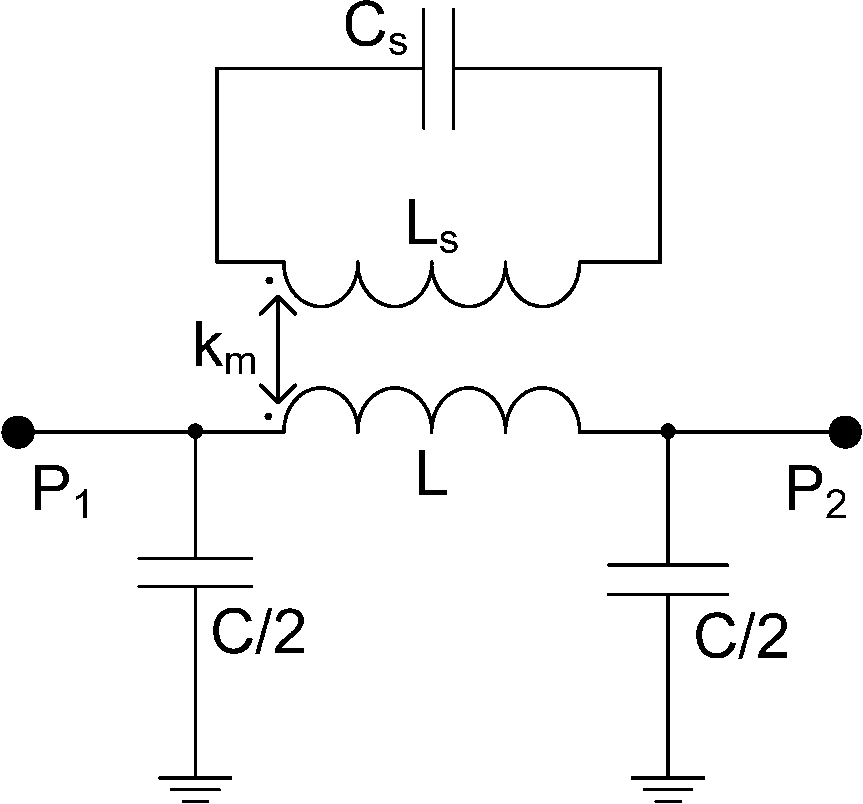
\includegraphics[scale=0.22]{fig2a}
\label{f2a}\label{f3e}}\hspace{0.3cm}
\subfigure[]{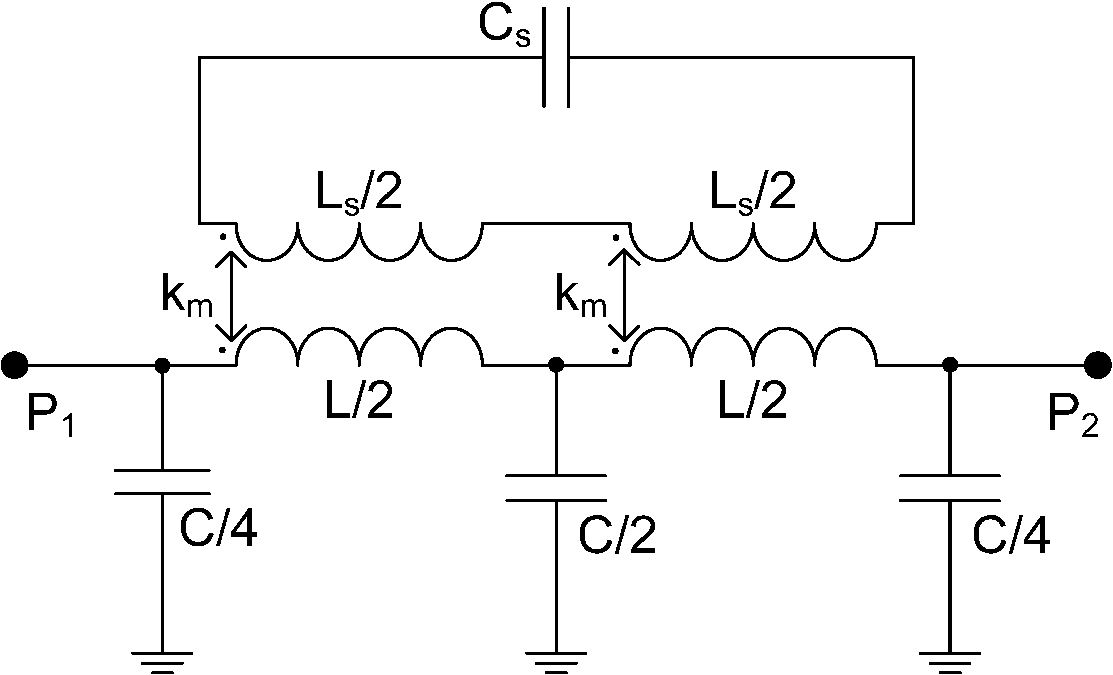
\includegraphics[scale=0.26]{fig2b}
\label{f2b}\label{f3f}}
\caption{Еквивалентна шема микрострип вода оптерећеног са СРР-ом, која има: (a) једну, и (b) две $\Pi$-ћелије.} 
\label{f2}
\end{figure}
Микрострип вод оптерећен СРР-ом са паралелним процепом ближе воду приказан је на \Fig{f1}, заједно са релевантним димензијама. Слична структура, али са двоструким СРР-овима, проучавана је у~\cite{bib16}, где је предложена еквивалентна шема приказана на \Fig{f2a}. Вод је представљен помоћу једне $\Pi$-ћелије. Овде се предлаже унапређени модел приказан на \Fig{f2b}, где је вод представљен помоћу две $\Pi$-ћелије. Биће демонстрирано да ово коло, које има исти број независних параметара као и претходно, омогућава много боље слагање са симулацијама и мерењима.

Како би се екстраховали параметри $L$ и $C$ вода (\Fig{f2}), узимајући у обзир спрегу између вода и најближе ивице СРР-а, систем је моделован као секција вишепроводничког вода. Програм LINPAR~\cite{bib19} је коришћен за нумеричко израчунавање квази-статичких параметара вода. Као излазни подаци добијају се матрице подужних индуктивности и капацитивности, из којих се могу добити параметри секција коначне дужине.

У складу са геометријом спреге између СРР-а и вода, проучаване структуре су подељене у пет група, приказаних у табели~\ref{tab1}. У функцији од оријентације СРР-а, микрострип вод је спрегнут са целом ивицом, или два њена дела раздвојена процепом.

\begin{table}[!t]
  \centering
 \caption{Конфигурације СРР-ова спрегнутих са микрострип водом и екстраховани параметри. Спрега је узета у обзир само у шрафираним секцијама. Референтне равни су обележене тачкастим линијама.} 
  \label{tab1}
\begin{tabular}{| m{0.5cm}  | V V | m{3cm} |}
	\hline
    (а) & 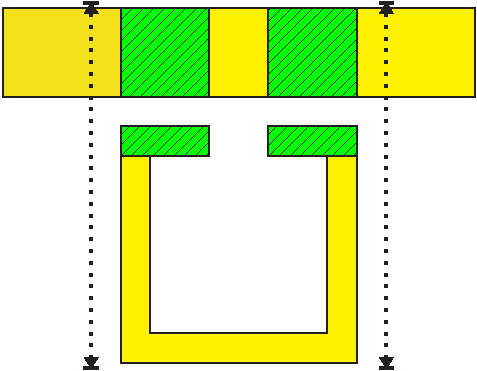
\includegraphics[width=\SirA,trim=0 0 0 -5]{pod0} &  
& \parbox[t]{3cm}{$L=1.51\,\mathrm{nH}$\\$C=0.72\,\mathrm{pF}$\\$L_s=7.97\,\mathrm{nH}$}  \\ \hline
    (б) & 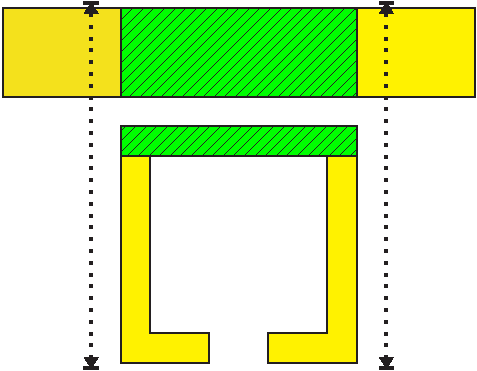
\includegraphics[width=\SirA,trim=0 0 0 -5]{pod180}& 
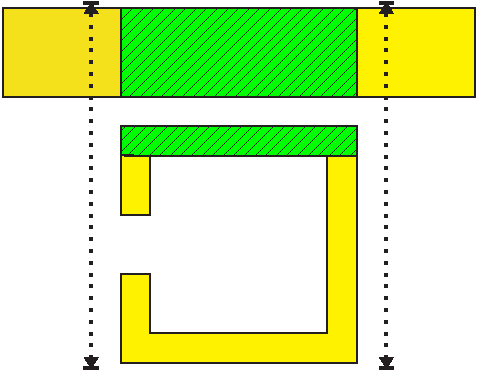
\includegraphics[width=\SirA,trim=0 0 0 -5]{pod90} 
& \parbox[t]{3cm}{$L=1.51\,\mathrm{nH}$\\$C=0.74\,\mathrm{pF}$\\$L_s=7.92\,\mathrm{nH}$} \\ \hline
    (в) & 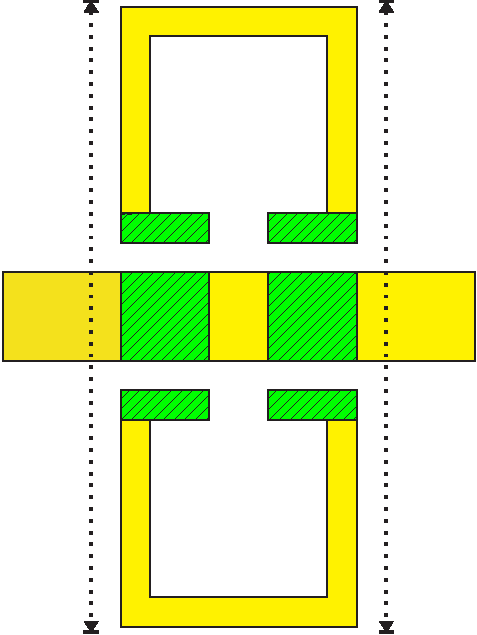
\includegraphics[width=\SirA,trim=0 0 0 -5]{pod0x2} &
& \parbox[t]{3cm}{$L=1.5\,\mathrm{nH}$\\$C=0.82\,\mathrm{pF}$\\$L_s=7.97\,\mathrm{nH}$} \\ \hline
    (г) & 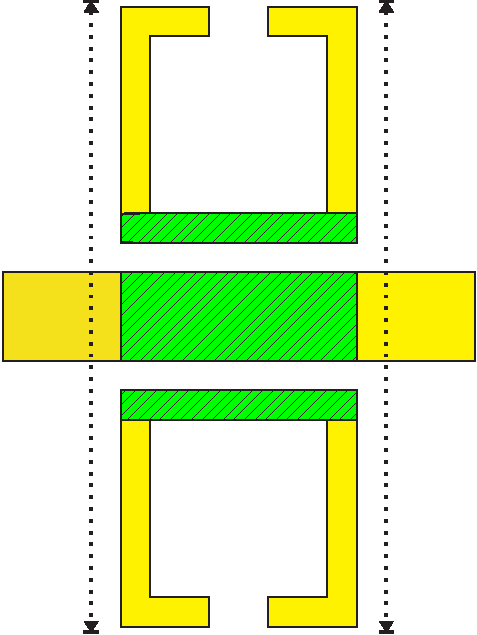
\includegraphics[width=\SirA,trim=0 0 0 -5]{pod180x2}& 
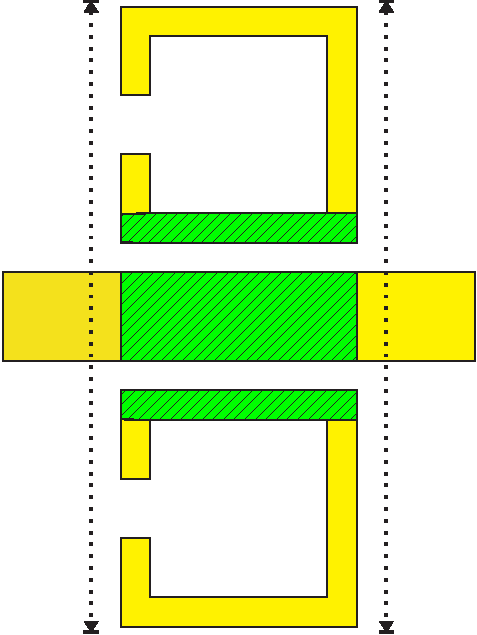
\includegraphics[width=\SirA,trim=0 0 0 -5]{pod90x2} 
& \parbox[t]{3cm}{$L=1.5\,\mathrm{nH}$\\$C=0.86\,\mathrm{pF}$\\$L_s=7.92\,\mathrm{nH}$} \\ \hline
    (д) & 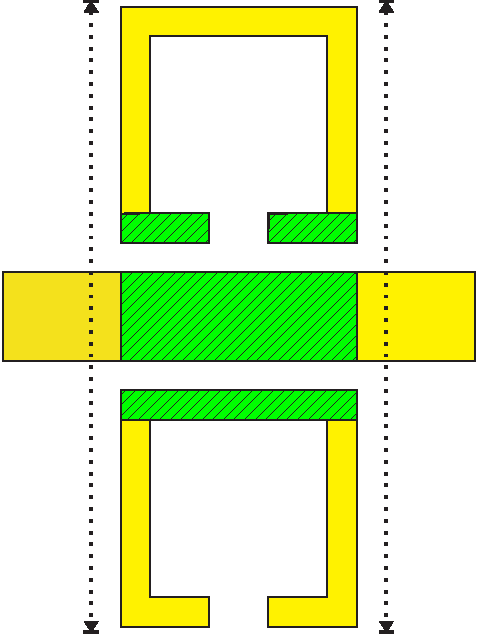
\includegraphics[width=\SirA,trim=0 0 0 -5]{pod180+pod0} & 
&
\parbox[t]{3cm}{$L=1.5\,\mathrm{nH}$\\$C=0.84\,\mathrm{pF}$\\$L_{s1}=7.97\,\mathrm{nH}$\\$L_{s2}
=7.92\,\mathrm{nH}$} \\ \hline
  \end{tabular}
%\vspace{1em}
\end{table}
У табели~\ref{tab1} могу се разликовати три врсте означених секција: изоловане, и спрегнуте са једном или две ивице СРР-а. Параметри сваке секције су прорачунати коришћењем подужних вредности. Резултирајући параметри вода (дати у трећој колони табеле) добијени су сабирањем параметара индивидуалних секција. Може се видети да је индуктивност вода, $L$, врло слична у свим конфигурацијама, док капацитивност, $C$, више варира (око 15\%) у зависности од спреге. Индуктивности прстенова, $L_S$, састоје се од два дела: 1) од секције која је спрегнута са водом, која се прорачунава на основу одговарајућег елемента матрице, и 2) од изолованог вода, чија је дужина једнака преосталом, неспрегнутом делу СРР-а. Бредности $L_S$ дате у табели се нешто разликују због чињенице да спрегнута секција има нешто нижу вредност индуктивности. У наставку су усвојене исте вредности индуктивности, $L=1.5\, \mathrm{nH}$ и $L_S = 8\, \mathrm{nH}$, за све разматране конфигурације.

\section{Екстракција параметара кола на основу симулираних резултата}

Откривено је да се различите конфигурације микрострип вода спрегнутог са СРР-овима могу моделовати истом топологијом кола, само са различитим вредностима параметара. На основу топологије, све разматране конфигурације могу се поделити у три категорије:
\begin{itemize}
\item СРР са процепом паралелним воду или два СРР-а са паралелним процепима, симетричним у односу на вод,
\item два СРР-а са паралелним процепима, при чему је један процеп ближе а други даље од вода,
\item један или два СРР-а са нормалним процепима.
\end{itemize}
За сваку топологију, могу се извести аналитички изрази за резонантну фреквенцију и фреквенцију минимума рефлексије. Ови изрази ће бити искоришћени за одређивање преосталих параметара (коефицијент магнетне спреге, $k_m$, капацитивност СРР-а, $C_s$), полазећи од фреквенција добијених у нумеричким симулацијама. Једини параметар који је неопходно фитовати је коефицијент електричне спреге, $k_e$; односно међусобна капацитивност, $C_m=k_e \sqrt{CC_s }$, у случају СРР-ова са нормалним процепима (овај коефицијент је уведен у секц.~\ref{sec:ML2SPerp}). 

\subsection{СРР са процепом паралелним воду}\label{sec3:2}
Микрострип водови оптерећени са СРР-овима са паралелним процепом приказани су на \Fig{f3}.
Параметри еквивалентне шеме $L$, $C$ и $L_S$ дати су у табели~\ref{tab1} за све конфигурације са \Fig{f3} (они зависе од геометрије и карактеристика материјала). Преостали параметри, $C_S$ и $k_m$, ће бити одређени на основу $Ѕ$-параметара добијених симулацијом. Треба приметити да, у разматраном фреквенцијском опсегу, симулирани $Ѕ_{11}$ параметар поседује само један минимум испод резонантне учестаности, док еквивалентне шеме поседују два минимума: један испод и један изнад резонансе. Присуство овог паразитног минимума смањује опсег у коме је могуће добити добро слагање између симулације и еквивалентне шеме. Ипак, шема са две П-ћелије [\Fig{f2b}] помера овај минимум на више учестаности у односу на модел са једном ћелијом, о чему ће се дискутовати касније.
%\begin{figure}[!t]
%\subfigure[]{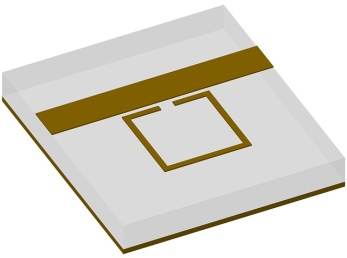
\includegraphics[width=2cm]{fig3a}
%\label{f3a}}
%\subfigure[]{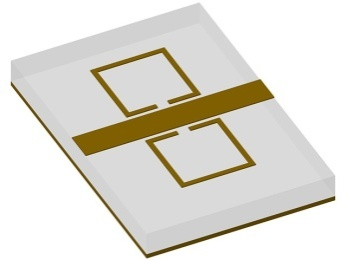
\includegraphics[width=2cm]{fig3b}
%\label{f3b}}
%\addtocounter{subfigure}{2}
%\subfigure[]{\includegraphics[scale=0.18]{fig3e}
%\label{f3e}}
%\addtocounter{subfigure}{-3}
%\subfigure[]{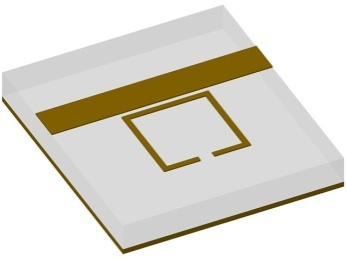
\includegraphics[width=2cm]{fig3c}
%\label{f3c}}
%\subfigure[]{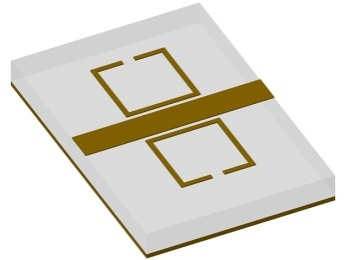
\includegraphics[width=2cm]{fig3d}
%\label{f3d}}
%\addtocounter{subfigure}{1}
%\subfigure[]{\includegraphics[scale=0.18]{fig3f}
%\label{f3f}}
%\caption{Microstrip line loaded with SRRs with gaps parallel to the line: (a) one SRR with gap
%near the line, (b) two SRRs with gaps near the line, (c) one SRR with gap far from the line,
%(d) two SRRs with gaps far from the line. These configurations can be modeled by the
%equivalent circuits (e) and (f).}
%\label{f3}
%\end{figure}
\begin{figure}[!t]
\centering
\begin{tabular}{W W}
\subfigure[]{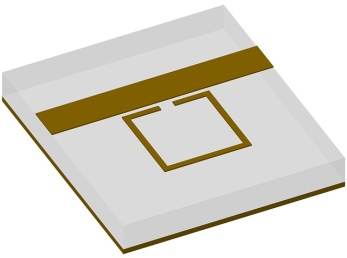
\includegraphics[width=\linewidth]{fig3a}
\label{f3a}} &
\subfigure[]{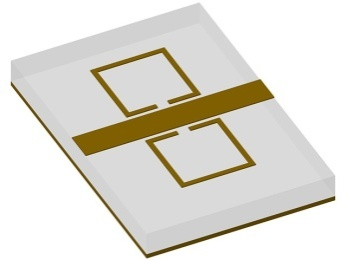
\includegraphics[width=\linewidth]{fig3b}
\label{f3b}} \\
%\addtocounter{subfigure}{2}
%\subfigure[]{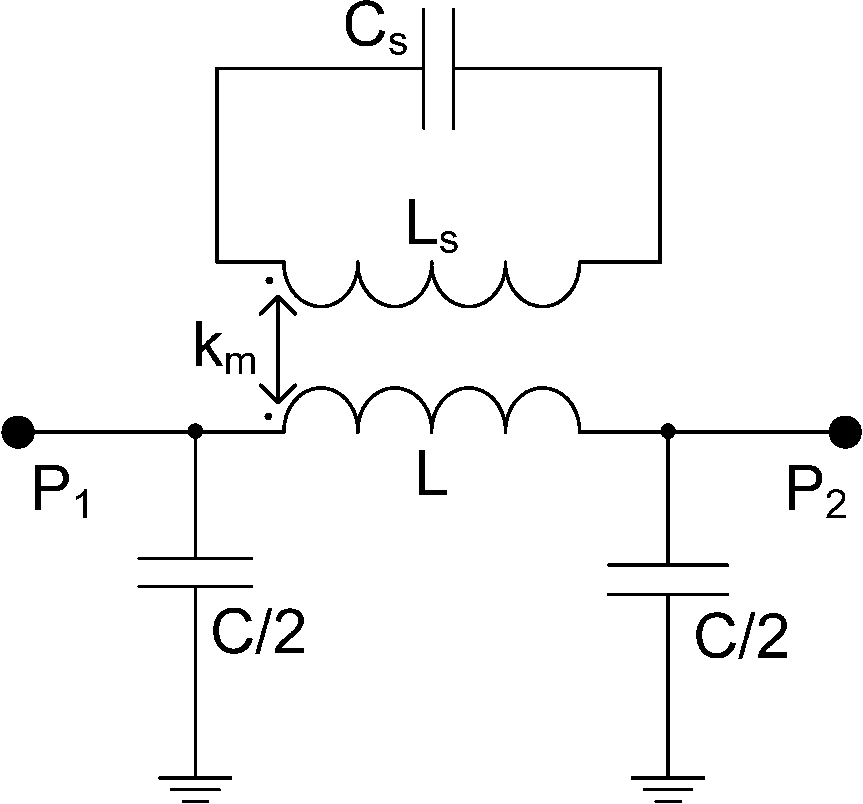
\includegraphics[width=0.75\linewidth]{fig2a}
%\label{f3e}} \\
%\addtocounter{subfigure}{-3}
\subfigure[]{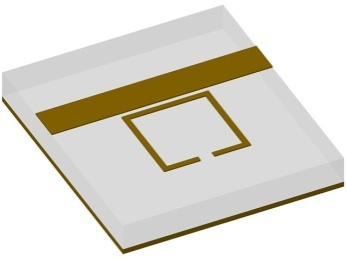
\includegraphics[width=\linewidth]{fig3c}
\label{f3c}} &
\subfigure[]{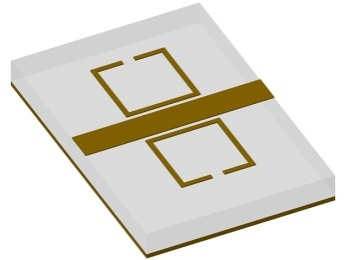
\includegraphics[width=\linewidth]{fig3d}
\label{f3d}} 
%\addtocounter{subfigure}{1}
%\subfigure[]{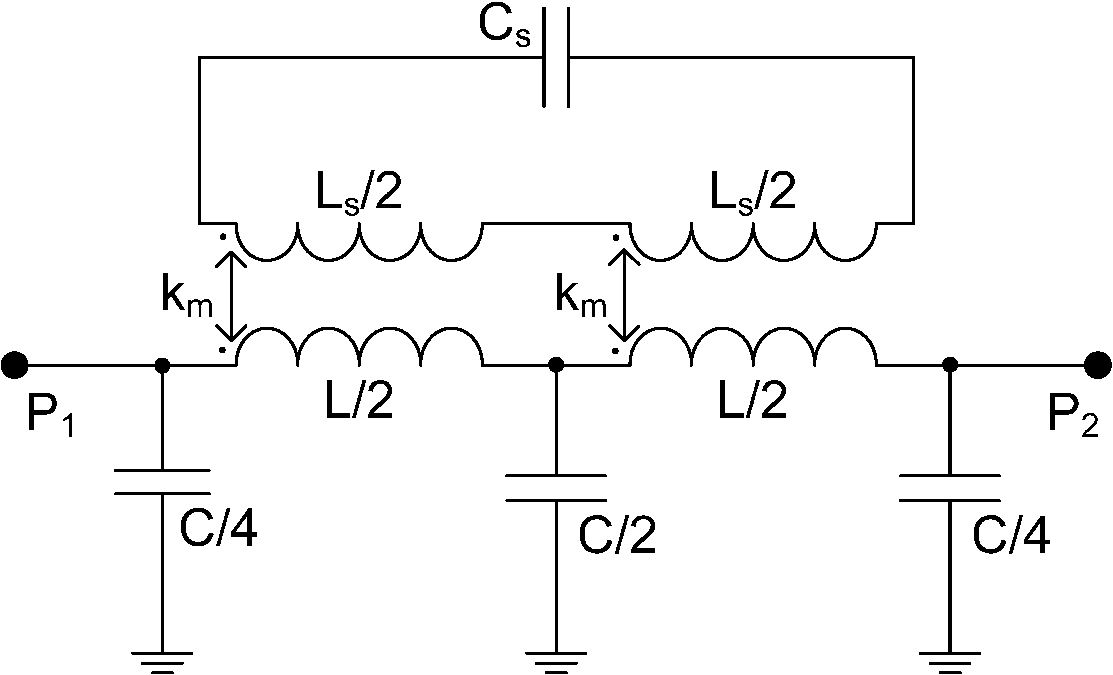
\includegraphics[width=\linewidth]{fig2b}
%\label{f3f}}
\end{tabular}
\caption{Микрострип вод спрегнут са СРР-овима са паралелним процепима: (а) један СРР са процепом ближе воду, (б) два СРР-а са процепима даље од вода.} 
\label{f3}
\end{figure}

Капацитивност $C_S$ се добија из резонантне учестаности СРР-а $f_r=\omega_r/2\pi$ на следећи начин:
\begin{equation}
f_r = \frac{1}{2\pi \sqrt{L_SC_S}}\;.
\end{equation}

%%%%%%%%%%%%%%%%%%%%%%%%%%%%%%%%%%%%%%%%%%%%%%%%%%%%%%%%%%%%%%%%%%%%%%%%%%%%%%%%%%%%%
\subsubsection{Минимум $S_{11}$ испод резонансе}
%%%%%%%%%%%%%%%%%%%%%%%%%%%%%%%%%%%%%%%%%%%%%%%%%%%%%%%%%%%%%%%%%%%%%%%%%%%%%%%%%%%%%

Коефицијент магнетне спреге, $k_m$, се одређује на основу првог минимума $S_{11}$, $f_\text{min}=\omega_\text{min}/2\pi$,  за коло са \Fig{f2}. Како би се поједноставило израчунавање, биће примењена Бартлетова бисекциона теорема~\cite{bib20}. Коефицијент $k_m$ се онда добија као функција $f_\text{min}$, резонантне фреквенције$f_r$ и параметара вода $L$ и $C$,
\begin{equation}
k_m^2 = \left( 1 - \frac{\omega_r^2}{\omega_\text{min}^2} \right) \left( 1 - a_{1,2} \right) 
\end{equation}
где $a_1$ одговара колу са једном ћелијом [\Fig{f2a}], а $a_2$ колу са две ћелије [\Fig{f2b}]. Ови коефицијенти су дати са
\begin{align}
a_1 & = \left[ \frac{L}{C}Y_0^2 + 2b \right]^{-1} \\
a_2 & = \left[ \frac{L}{C}Y_0^2 \left( 1 - \frac{b}{2-b} \right) + b \right]^{-1} 
\end{align}
где је $Y_0$ карактеристична адмитанса вода ($20\,\mathrm{mS}$ у овом случају), и 
\begin{equation*}
b  = \left( \frac{\omega_\text{min}}{\omega_0} \right)^2;\quad
\omega_0^2=\frac{8}{LC}\;.
\end{equation*}
%%%%%%%%%%%%%%%%%%%%%%%%%%%%%%%%%%%%%%%%%%%%%%%%%%%%%%%%%%%%%%%%%%%%%%%%%%%%%%%%%%
\begin{figure}[!t]\centering
\subfigure[]{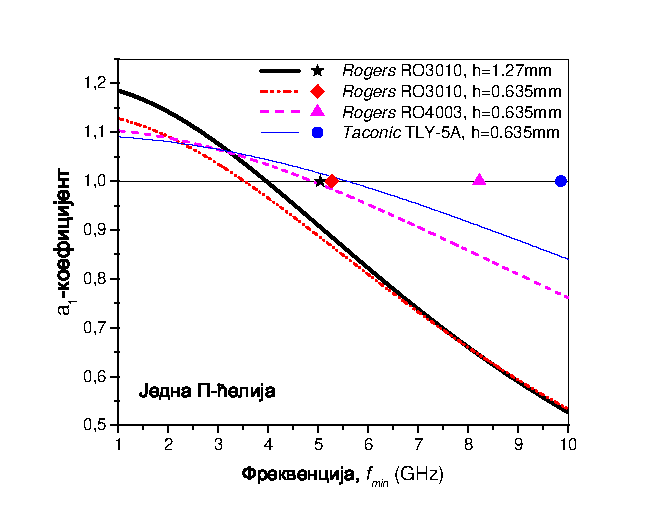
\includegraphics[width=0.8\textwidth]{enhmod_slike/fig4a}
\label{f4a}}
\subfigure[]{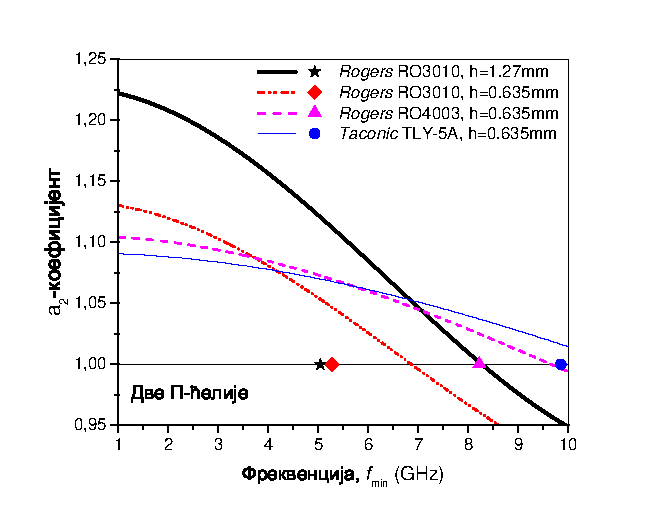
\includegraphics[width=0.8\textwidth]{enhmod_slike/fig4b}
\label{f4b}}
\caption{Поређење коефицијената $a$ за еквивалентну шему са (а) једном (б) две П-ћелије за случај са \Fig{f3a}. Хоризонталне црне линије означавају вредност 1 на вертикалној оси, а маркери означавају фреквенције минимума $S_{11}$ за одговарајуће супстрате. За $k_m \in \mathbb{R}$ потребно је $a_{1,2}>1$.}
\label{f4}
\end{figure}
%%%%%%%%%%%%%%%%%%%%%%%%%%%%%%%%%%%%%%%%%%%%%%%%%%%%%%%%%%%%%%%%%%%%%%%%%%%%%%%%%%

3Д електромагнетне симулације и мерења за све структуре са \Fig{f3} показују да се минимум
$S_{11}$ јавља пре резонансе СРР-а, $f_r$, због чега је прва заграда у (2) негативна. Како би се добила реална вредност коефицијента спреге $k_m$, (која омогућава слагање фреквенција првог минимума $S_{11}$ добијених из еквивалентне шеме и симулације), неопходно је да десна страна једначине буде позитивна, што захтева $a_{1,2}>1$. 

На сл.~\ref{f4a} и \ref{f4b} приказано је поређење коефицијената $a$ израчунатих за шеме са једном и две ћелије, респективно, за СРР спрегнут са 50-омским микрострип водом [\Fig{f3a}] на различитим супстратима. На основу позиције минимума $S_{11}$ (одговарајући маркери), може се видети да услов $a>1$ није задовољен ни за један случај са \Fig{f4a}. С друге стране, услов је испуњен за све случајеве са \Fig{f4b}. Такође, супстрат са највећом пермитивношћу (Rogers RO3010) испољава најнижу горњу границу опсега у ком $k_m$ има реалну вредност (3.51 GHz за једну ћелију и 7.02 GHz за две). Треба приметити да коефицијент $a$ није функција параметара СРР-а, већ само фреквенције минимума $S_{11}$ и параметара вода.

Сл.~\ref{f4a} и \ref{f4b} јасно показују важну предност унапређеног модела структуре, у поређењу са шемом са једном П-ћелијом, а то је два пута већи опсег у ком $k_m$ има реалне вредности.

Уколико би уземљење преко вије било присутно, добио би се одзив пропусника опсега, и минимум $S_{11}$ би се појавио изнад трансмисионе нуле у симулацијама. У том случају, добро слагање може се добити помоћу шеме са једном ћелијом~\cite{bib16}. Тада би овде предложена шема била врло слична моделу пријављеном у~\cite{bib13}, где је једна ћелија модификована како би се омогућило централно позиционирање индуктивности вије.

%%%%%%%%%%%%%%%%%%%%%%%%%%%%%%%%%%%%%%%%%%%%%%%%%%%%%%%%%%%%%%%%%%%%%%%%%%%%%%%%%%%%%
\subsubsection{Минимум $S_{11}$ изнад резонансе}
%%%%%%%%%%%%%%%%%%%%%%%%%%%%%%%%%%%%%%%%%%%%%%%%%%%%%%%%%%%%%%%%%%%%%%%%%%%%%%%%%%%%%

Обе еквивалентне шеме са \Fig{f2} испољавају други минимум $S_{11}$ изнад резонантне фреквенције СРР-а, који се не појављује у симулацијама или мерењима. Овај спуриозни ефекат је последица апроксимације дистрибуираног кола помоћу елемената са концентрисаним параметрима. Како би се повећао опсег у коме се еквивалентна шема може користити, неопходно је потиснути овај минимум ка што већим фреквенцијама. Ово се постиже коришћењем шеме са две ћелије.

Како би се разјаснио овај ефекат, почиње се од услова за идеално прилагођење (минимум $S_{11}$) за симетрично коло (следећи Бартлетову теоерему): $Y_\text{in,even} Y_\text{in,odd}=Y_0^2$, где се парна и непарна адмитанса одређују постављањем отворене везе, односно кратког споја у раван симетрије. После преуређења, услов се може преформулисати као
\begin{equation}
\frac{\omega_r^2 - \omega_\text{min}^2}{\omega_r^2-(1-k_m^2)\omega_\text{min}^2} =
a_{1,2}^{-1}
\end{equation}
где вредности $a_{1,2}$ одговарају изразима (3) и (4) за једну и две ћелије, респективно. На ниским учестаностима $a_2$ може се апроксимирати као $a_2^{-1} \approx
\frac{L}{C} Y_0^2 + \frac{b}{2}$. Поређењем овог израза са (3) примећује се да је коефицијент уз члан $b$ четири пута мањи. Пошто је $b$ пропорционално квадрату учестаности [видети (4)], ово имплицира да $a_2$ варира двоструко спорије са учестаношћу него $a_1$, због чега испољава фреквенцијску зависност ближу очекиваној за идеални вод (који би требало да има константну вредност коефицијента $a$). 
\begin{figure}[!t]
\centering
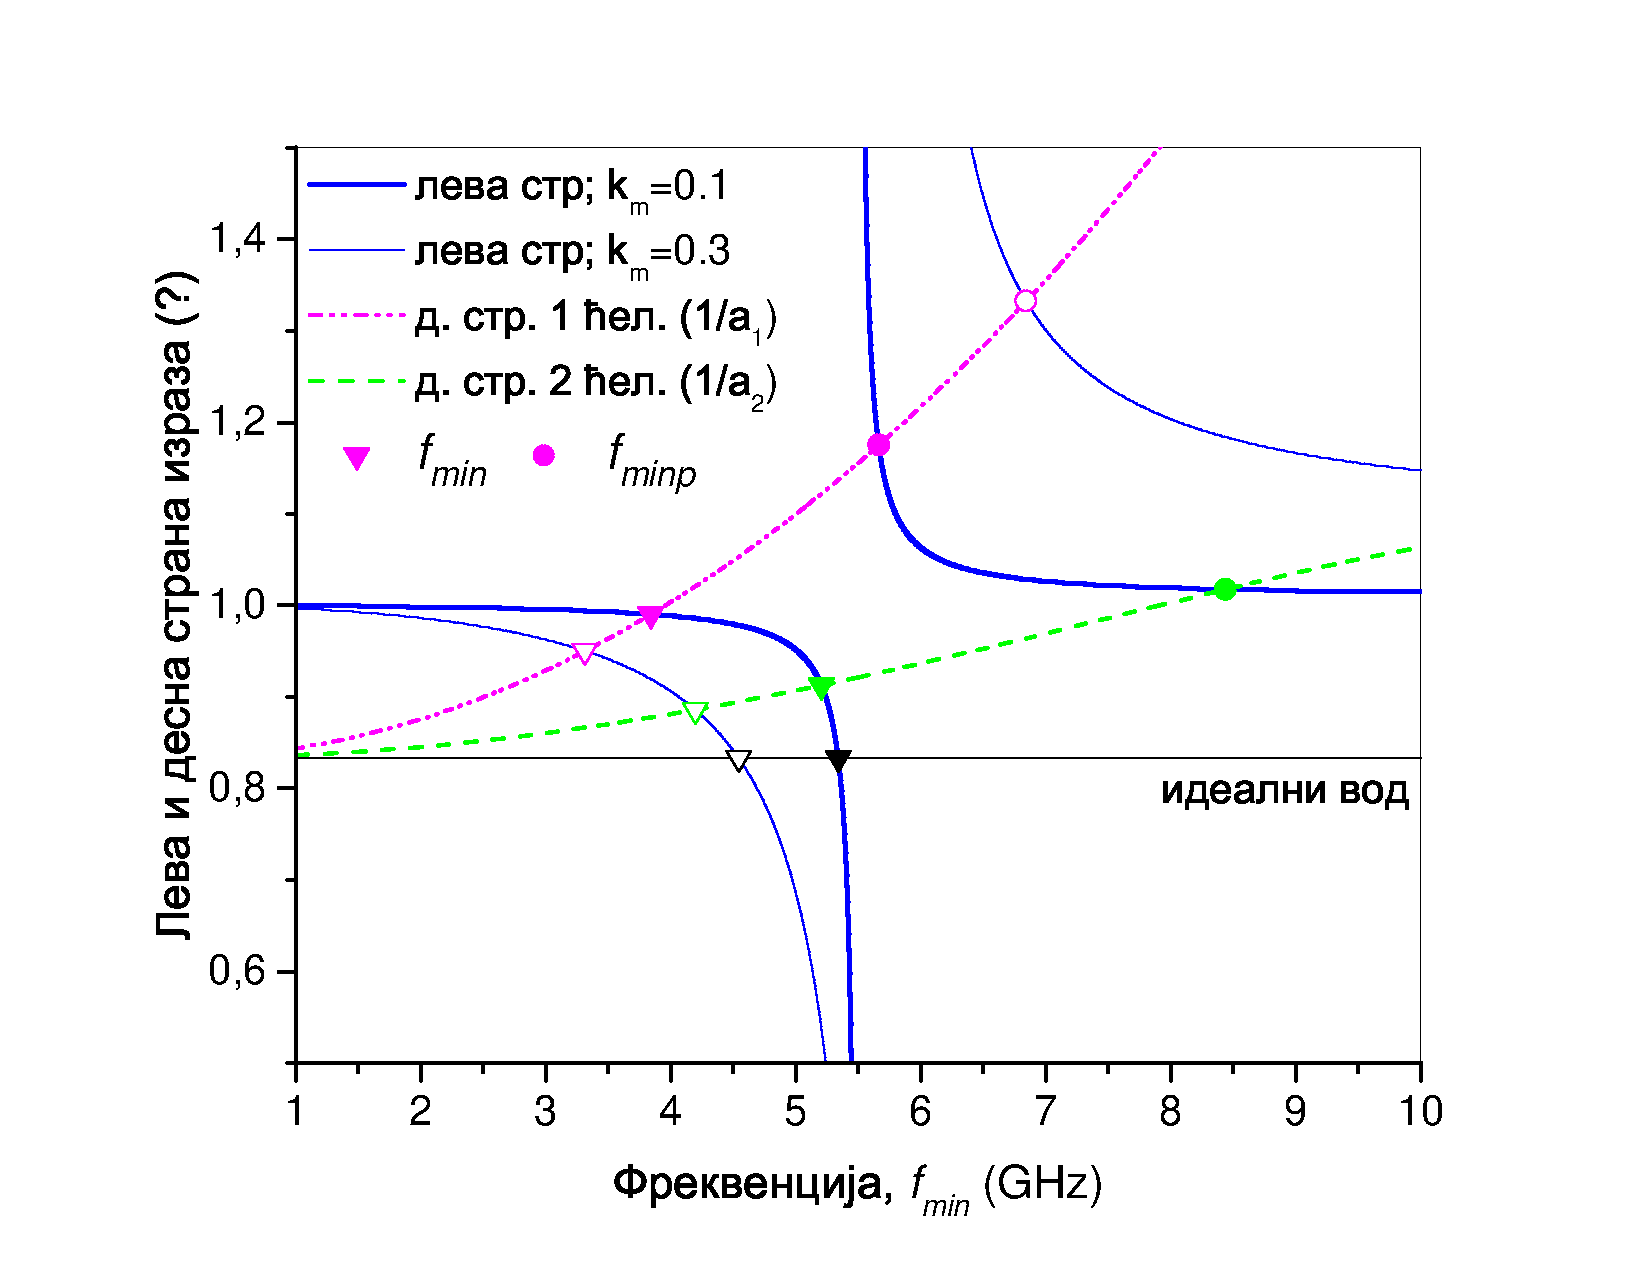
\includegraphics[width=\textwidth]{enhmod_slike/fig5}
\caption{График зависности леве (пуне линије) и десне (испрекидане линије) стране израза (5). Тачке пресека представљају минимуме $S_{11}$ за одговарајуће случајеве.}
\label{f5}
\end{figure}

На \Fig{f5} лева и десна страна израза (5) су приказане на једну и две ћелије и за два различита коефицијента спреге (параметри вода одговарају случају са \Fig{f3a}). Пресечне тачке одговарајућих кривих за леву и десну страну означавају решења (5) и, према томе, минимуме $Ѕ_{11}$. Пресечне тачке испод резонансе СРР-а су означене троугловима, док су оне изнад, обележене круговима, паразитни минимуми $f_\text{minp}$, одсутни у симулацијама. Лева страна ове једначине не зависи од броја ћелија, већ само од коефицијента спреге $k_m$ и резонансе $f_r$ (пуне линије). Повећањем јачине спреге, ова крива се ,,шири`` (упоредити дебље и тање линије на слици), тако да је могуће подесити фреквенције оба минимума $Ѕ_{11}$ у датом опсегу. Такође, десна страна зависи само од параметара вода $L$ и $C$ (који су у основи одређени избором супстрата и карактеристичне импедансе), и има драстично другачији нагиб за основно и унапређено коло. Са слике се јасно види да је десна страна израза, која одговара унапређеном колу, много повољнија што се тиче паразитног минимума, који се јавља на много вишим фреквенцијама. Конкретно, за мале вредности коефицијента спреге ($k_m\sim 0.1$), други минимум $Ѕ_{11}$ јавља се одмах иза резонансе СРР-а за коло са једном ћелијом, чиме се драстично смањује његов фреквенцијски опсег.

%%%%%%%%%%%%%%%%%%%%%%%%%%%%%%%%%%%%%%%%%%%%%%%%%%%%%%%%%%%%%%%%%%%%%%%%%%%%%%%%%%%%%
\subsubsection{Екстраховани параметри еквивалентног кола}
%%%%%%%%%%%%%%%%%%%%%%%%%%%%%%%%%%%%%%%%%%%%%%%%%%%%%%%%%%%%%%%%%%%%%%%%%%%%%%%%%%%%%

Екстраховани параметри за коло са две ћелије [\Fig{f3f}] дати су у табели~\ref{tab2} за све конфигурације са \Fig{f3}.
\begin{table}[!t]
% increase table row spacing, adjust to taste
\renewcommand{\arraystretch}{1.3}
% if using array.sty, it might be a good idea to tweak the value of
% \extrarowheight as needed to properly center the text within the cells
\caption{Екстраховани параметри за кофигурације са \Fig{f3}.}
\label{tab2}
\centering
% Some packages, such as MDW tools, offer better commands for making tables
% than the plain LaTeX2e tabular which is used here.
\begin{tabular}{|l|c|c|c|c|c|}
\hline
модел & $f_r$(GHz) & $f_\text{min}$(GHz) & $C$(pF) & $C_S$(pF) & $k_m$ \\
\hline
\Fig{f3a} & 5.47 & 5.04 & 0.72 & 0.107 & 0.14 \\
\hline
\Fig{f3b} & 5.48 & 5.14 & 0.82 & 0.106 & 0.167 \\
\hline
\Fig{f3c} & 6.19 & 4.84 & 0.74 & 0.084 & 0.28 \\
\hline
\Fig{f3d} & 6.14 & 4.72 & 0.86 & 0.088 & 0.41 \\
\hline
\end{tabular}
\end{table}
Разлика у $C_S$ је услед другачијих резонантних учестаности, у складу са (1). Коефицијент спреге $k_m$ више варира, и значајно је већи за структуре без процепа у најближој ивици, где је спрега најизраженија. 

\subsection{\label{sec:ML2SP}
Микрострип вод спрегнут са два СРР-а са асиметричним процепима}
\begin{figure}[!t]
\subfigure[]{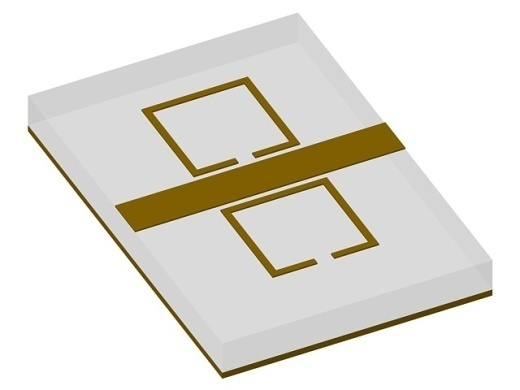
\includegraphics[width=0.48\columnwidth]{fig6a}
\label{f6a}}
\subfigure[]{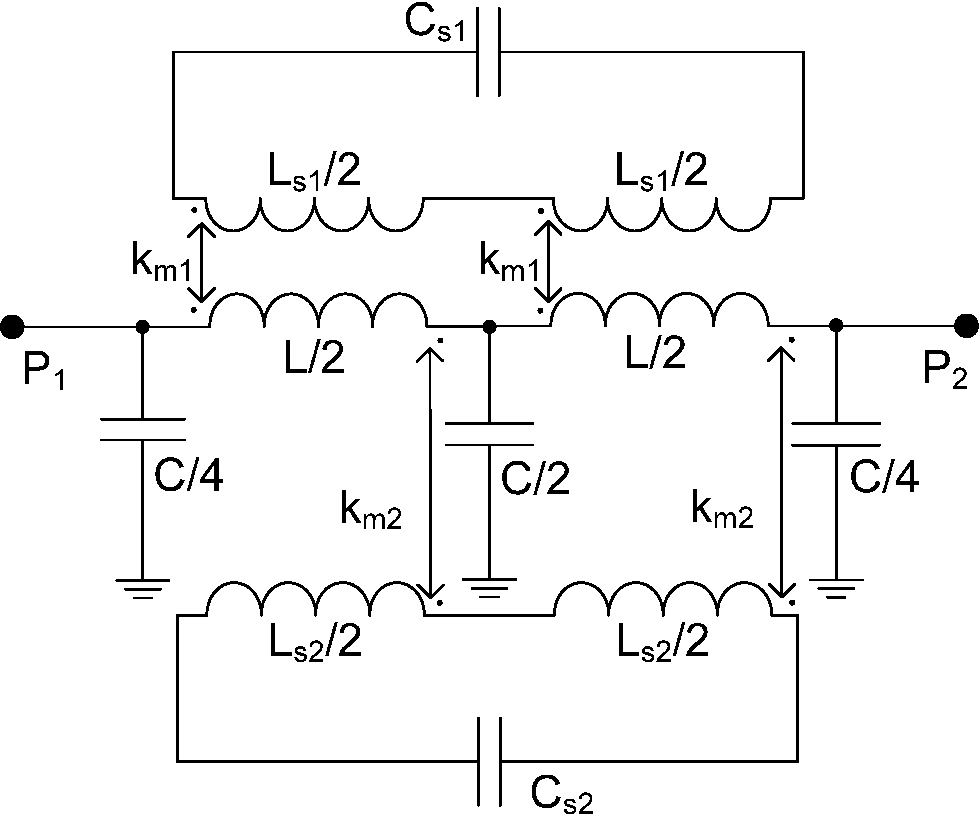
\includegraphics[width=0.48\columnwidth]{fig6b}
\label{f6b}}
\caption{(a) Микрострип вод спрегнут са два СРР-а са асиметричним процепима и (б) одговарајућа еквивалентна шема.}
\label{f6}
\end{figure}
Микрострипи вод са два асиметрична СРР-а, где је један процеп на ближој а други на даљој ивици [\Fig{f6a}] има компликованију еквивалентну шему [\Fig{f6b}] него у претходном случају. Она је суперпозиција две шеме са \Fig{f3f}, зато што СРР-ови имају различите спреге и резонантне фреквенције. 

Вредности екстрахованих параметара $C_{s1}=0.105\, \mathrm{pF}$ и $C_{s2}=0.081\,
\mathrm{pF}$ одређене су на основу резонантних фреквенција $f_{r1}$ и $f_{r2}$, добијених симулацијом.

Коефицијент магнетне спреге $k_{m1,2}$  одређен је применом Бартлетове теореме на коло са \Fig{f6b}, на сличан начин као и за \Fig{f2b}. Да би се добили $k_{m1,2}$ треба решити следећи систем (пошто постоје два минимума $S_{11}$, $f_\text{min1,2}$):
\begin{equation}
\begin{split}
\frac{\omega_\text{min1}^2}{\omega_{r1}^2-\omega_\text{min1}^2}k_{m1}^2 +
\frac{\omega_\text{min1}^2}{\omega_{r2}^2-\omega_\text{min1}^2}k_{m2}^2 = & a_2^{(1)} -1, \\
\frac{\omega_\text{min2}^2}{\omega_{r1}^2-\omega_\text{min2}^2}k_{m1}^2 +
\frac{\omega_\text{min2}^2}{\omega_{r2}^2-\omega_\text{min2}^2}k_{m2}^2 = & a_2^{(2)} -1;
\end{split}
\end{equation}
где су $a_2^{(1),(2)}$ израчунати на основу (4). Коначно, добија се $k_{m1}=0.14$ и $k_{m2}=0.26$.

За еквивалентну шему са једном ћелијом, систем (6) остаје исти, осим што је потребно заменити $a_2$ са $a_1$, израчунатим на основу (3). У том случају, прва једначина у (6) одговара првом минимуму $S_{11}$ испод резонансе. Дакле, коефицијенти на левој страни биће позитивни, док је десна страна негативна, па једначина нема решења. Последично, немогуће је поклопити први минимум у симулацији/мерењу и еквивалентној шеми. Други минимум, међутим, налази се између резонанси, зато је један од коефицијената на левој страни (6) негативан, па је могуће извршити поклапање. Онда важи следећа релација између коефицијената спреге:
\begin{equation}
k_{m1}^2 = \left(\omega_\text{min2}^2-\omega_{r1}^2 \right) \left(\frac{k_{m2}^2}{\omega_{r2}^2-\omega_\text{min2}^2 } - \frac{a_1^{(2)}-1}{\omega_\text{min2}^2}\right).
\end{equation}
При решавању (7), треба узети у обзир да $k_{m2}$
(који одговара СРР-у са даљим процепом) треба бити веће од $k_{m1}$. 

\subsection{\label{sec:ML2SPerp} 
Микрострип вод спрегнут са СРР-овима са нормалним процепима}
%%%%%%%%%%%%%%%%%%%%%%%%%%%%%%%%%%%%%%%%%%%%%%%%%%%%%%%%%%%%%%%%%%%%%%%%%%%%%
\begin{figure}[!t]
\centering
\subfigure[]{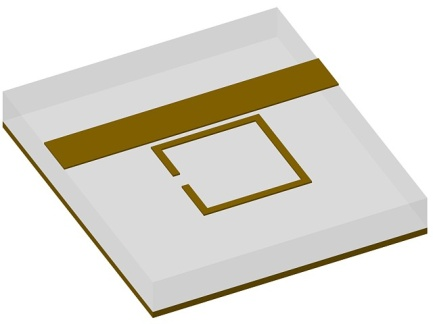
\includegraphics[width=0.4\columnwidth]{fig7a}
\label{f7a}}\hfil
\subfigure[]{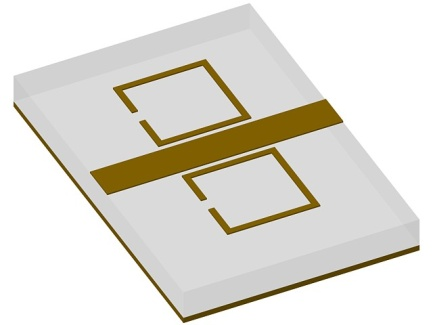
\includegraphics[width=0.4\columnwidth]{fig7b}
\label{f7b}}
\subfigure[]{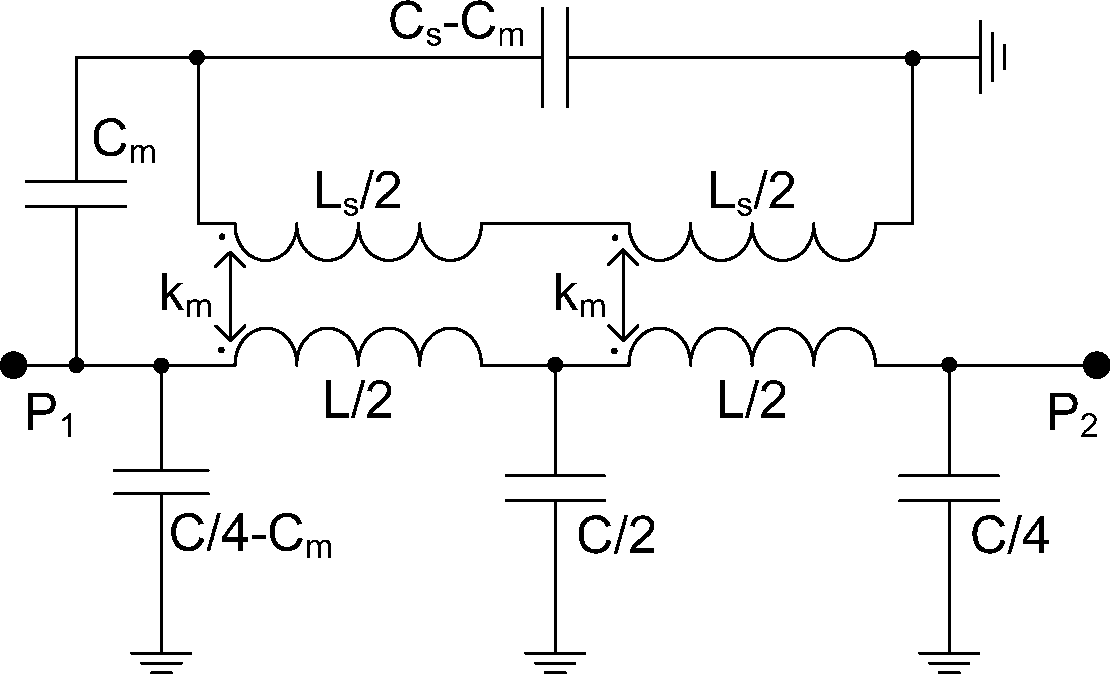
\includegraphics[width=0.6\columnwidth]{fig7c}
\label{f7c}}
\caption{СРР-ови са процепима нормалним у односу на вод: (а) један СРР,
(б) два СРР-а симетрично у односу на вод; оба случаја се могу моделовати истим еквивалентними колом (в).} 
\label{f7}
\end{figure}
%%%%%%%%%%%%%%%%%%%%%%%%%%%%%%%%%%%%%%%%%%%%%%%%%%%%%%%%%%%%%%%%%%%%%%%%%%%%%
СРР-ови приказани на \Fig{f7} разликују се од претходних конфигурација, утолико што су заротирани за 90 степени, што значи да цела структура више није симетрична у односу на микрострип вод. У овом случају, електрично поље вода паралелно је у односу на процеп, што узрокује додатну електричну спрегу, укључену у еквивалентну шему приказану на \Fig{f7c}.

Микрострип вод, оптерећен са једним СРР-ом са нормалним процепом [\Fig{f7a}], има исту еквивалентну шему као и два СРР-а симетрично постављена с обе стране [\Fig{f7b}], само са различитим вредностима параметара.

Вредности одговарајућих елемената кола $L$, $C$ и $L_S$ дате су у табели~\ref{tab1} за конфигурације са \Fig{f7}. Коефицијент магнетне спреге $k_m$ за структуре са сл.~\ref{f7a} и \ref{f7b} апроксимиране су вредностима добијеним за одговарајуће СРР-ове са процепима паралелним и даље од вода [\Fig{f3c} и \ref{f3d}, респективно], пошто они имају веома сличну расподелу струје. Преостали параметри, $C_S$ и $C_m$, су одређени коришћењем резонантне учестаности ($C_S$ се добија као функција од $C_m$, које се изводи помоћу процедуре фитовања са симулацијом).

%%%%%%%%%%%%%%%%%%%%%%%%%%%%%%%%%%%%%%%%%%%%%%%%%%%%%%%%%%%%%%%%%%%%%%%%%%%%%%
\begin{figure}[!t]
\centering
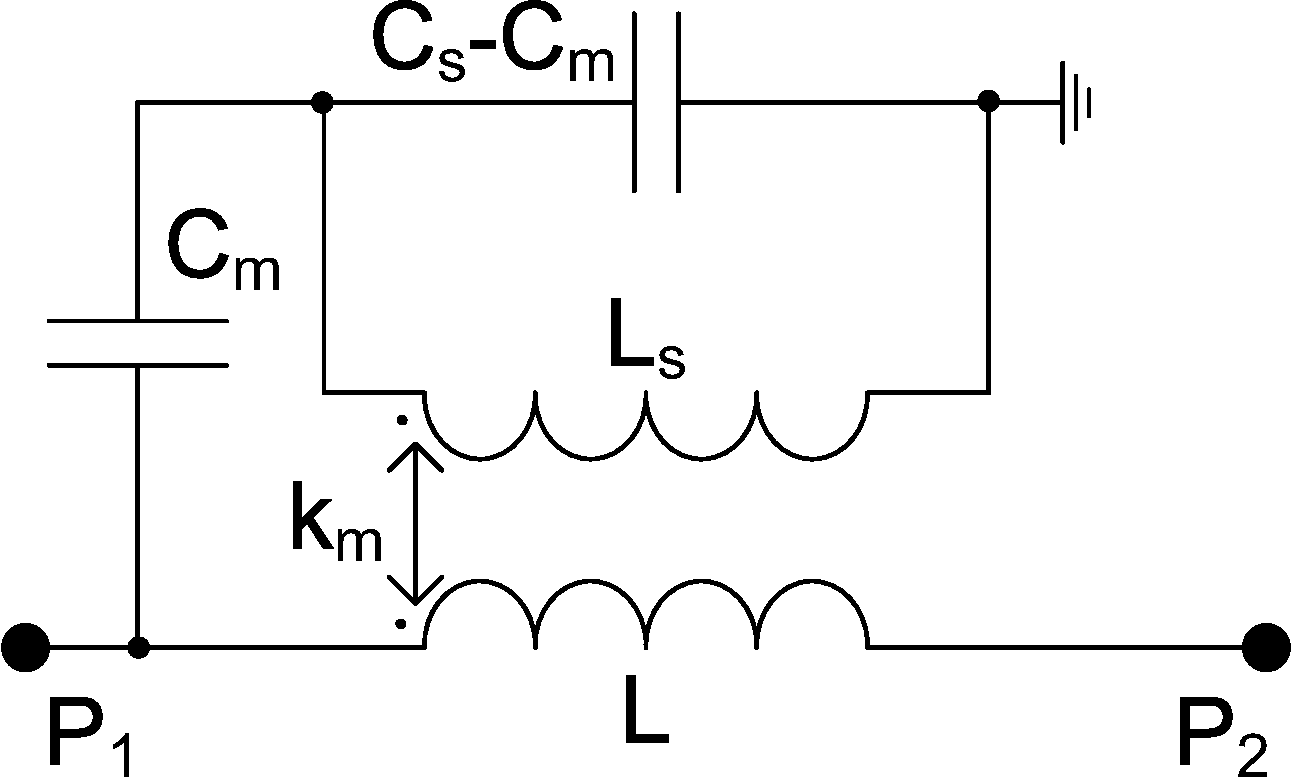
\includegraphics[width=0.4\columnwidth]{fig8}
\caption{Поједностављена шема за рачунање резонантне учестаности.}
\label{f8}
\end{figure}
%%%%%%%%%%%%%%%%%%%%%%%%%%%%%%%%%%%%%%%%%%%%%%%%%%%%%%%%%%%%%%%%%%%%%%%%%%%%%%
Како би се одредила приближна резонантна фреквиенција (односно минимум $Ѕ_{21}$), биће коришћена шема са \Fig{f8}, на којој су паралелно везани кондензатори уклоњени, у поређењу са \Fig{f7c}. Ово значајно олакшава анализу, док је утицај на резонансу занемарљив.

Исписивањем система једначина на основу Кирхофових закона, добија се следећа матрична релација између струја и напона на портовима 1 и 2:
\begin{multline}\label{mat8}
\begin{bmatrix}
j\omega (1-L_S/L_m) & 1 \\
\dfrac{j}{\omega L_m}(1-\omega^2 L_S C_S) + j\omega C_m & 0
\end{bmatrix}
\begin{bmatrix} V_1 \\ I_1 \end{bmatrix}  \\  = 
\begin{bmatrix}
-j\omega C_m L_S/L_m & 1 - \omega^2 L_m C_m (1/k_m^2 -1) \\
\dfrac{j}{\omega L_m}(1-\omega^2 L_S C_S) & \dfrac{L}{L_m}(1-\omega^2 L_S C_S(1-k_m^2))
\end{bmatrix}
\begin{bmatrix} V_2 \\ I_2 \end{bmatrix}\;.
\end{multline}
Услов за резонансу, односно непостојање трансмисије између портова, може се преформулисати као захтев да имамо нетривијално решење на левој страни, када је $V_2,I_2=0$ (тј. десна страна је једнака нули), што може бити испуњено само ако је детерминанта матрице на левој страни једнака нули:
\begin{equation}
\frac{j}{\omega L_m}(1-\omega^2 L_S C_S) + j\omega C_m
= \frac{j}{\omega L_m}(1-\omega^2 L_S C_S+\omega^2 L_m C_m)=0
\end{equation}
што даје следећу резонантну фреквенцију:
\begin{equation}
f_r = \frac{1}{2\pi\sqrt{L_S C_S - L_mC_m}} 
\end{equation}
са $L_m=k_m\sqrt{LL_S}$. 
Може се показати да, услед реципрочности ($S_{12}=S_{21}$), матрице на левој и десној страни (\ref{mat8}) једнаке, али у овом случају је једноставније разматрати ону на левој страни.

\begin{table}[!t]
% increase table row spacing, adjust to taste
\renewcommand{\arraystretch}{1.3}
% if using array.sty, it might be a good idea to tweak the value of
% \extrarowheight as needed to properly center the text within the cells
\caption{Екстраховани параметри за конфигурације са \Fig{f7}.}
\label{tab3}
\centering
% Some packages, such as MDW tools, offer better commands for making tables
% than the plain LaTeX2e tabular which is used here.
\begin{tabular}{|l|c|c|c|c|c|}
\hline
Конфигурације & $f_r$(GHz) & $C$(pF) & $C_S$(pF) & $k_m$ & $C_m$(pF) \\
\hline
\Fig{f7a} & 5.8 & \textbf{0.74} & 0.102 & \textbf{0.29} & \textbf{0.055} \\
\hline
\Fig{f7b} & 5.86 & \textbf{0.86} & 0.108 & \textbf{0.42} & \textbf{0.08} \\
\hline
\end{tabular}
\end{table}
Екстраховане вредности елемената кола (табела~\ref{tab3}) добијене су после мале оптимизације параметара $C_s$, $C_m$ и $k_m$, потребне због анализе поједностављеног кола. Може се видети да су вредности $L$, $C_s$ и $L_s$ веома сличне за обе структуре, док се $C$, $C_m$ и $k_m$ разликују. Разлика у $C_m$ и $k_m$ последица је јаче спреге са два СРР-а.

%%%%%%%%%%%%%%%%%%%%%%%%%%%%%%%%%%%%%%%%%%%%%%%%%%%%%%%%%%%%%%%%%%%%%%%%%%%%%%%%%
\subsection{Каскадиране структуре}
%%%%%%%%%%%%%%%%%%%%%%%%%%%%%%%%%%%%%%%%%%%%%%%%%%%%%%%%%%%%%%%%%%%%%%%%%%%%%%%%%

%%%%%%%%%%%%%%%%%%%%%%%%%%%%%%%%%%%%%%%%%%%%%%%%%%%%%%%%%%%%%%%%%%%%%%%%%%%%%%%%%
\begin{figure}[!t]\centering
\subfigure[]{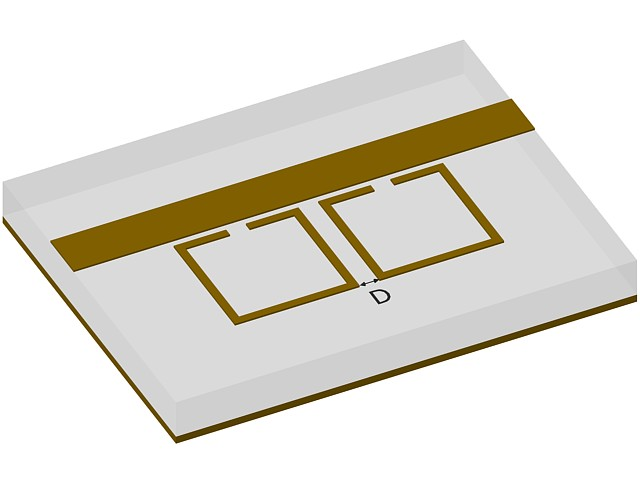
\includegraphics[width=0.55\columnwidth]{k2}
\label{fka}}
\subfigure[]{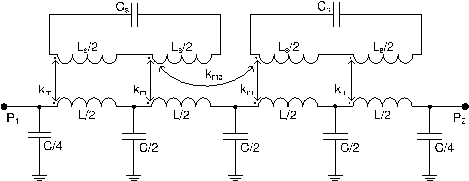
\includegraphics[width=0.9\columnwidth]{kaskada}
\label{fkb}}
\caption{(a) Каскадирани СРР-ови (б) одговарајуће еквивалентно коло.}
\label{fk}
\end{figure}
%%%%%%%%%%%%%%%%%%%%%%%%%%%%%%%%%%%%%%%%%%%%%%%%%%%%%%%%%%%%%%%%%%%%%%%%%%%%%%%%%
Јединичне ћелије, разматране горе, могу се каскадирати како би се добили филтри са унапређеним опсегом, као што је приказано на \Fig{fka} за СРР-ове са процепом паралелним и близу вода. Ова структуре се моделује еквивалентним колом са \Fig{fkb}, са претходно екстрахованим параметрима, и додатном спрегом између резонатора, која се одређује из симулације два резонатора, и може се користити за моделовање произвољног броја спрегнутих СРР-ова, све док се спрега између несуседних елемената може занемарити. Добијени коефицијенти спреге $k_{mc}$ за различита растојања између резонатора приказани су у табели~\ref{tabk}. 
%%%%%%%%%%%%%%%%%%%%%%%%%%%%%%%%%%%%%%%%%%%%%%%%%%%%%%%%%%%%%%%%%%%%%%%%%%%%%%%%%
\begin{table}[!t]
% increase table row spacing, adjust to taste
\renewcommand{\arraystretch}{1.3}
% if using array.sty, it might be a good idea to tweak the value of
% \extrarowheight as needed to properly center the text within the cells
\caption{Екстраховани коефицијент спреге између резонатора, $k_{mc}$.}
\label{tabk}
\centering
% Some packages, such as MDW tools, offer better commands for making tables
% than the plain LaTeX2e tabular which is used here.
\begin{tabular}{|l|c|c|c|c|c|}
\hline
$D$ (mm) & 0.1 & 0.2 & 0.3 & 0.4 & 0.5\\
\hline
$k_{mc}$ & 0.155 & 0.102 & 0.078 & 0.052 & 0.03\\
\hline
\end{tabular}
\end{table}
%%%%%%%%%%%%%%%%%%%%%%%%%%%%%%%%%%%%%%%%%%%%%%%%%%%%%%%%%%%%%%%%%%%%%%%%%%%%%%%%%

%%%%%%%%%%%%%%%%%%%%%%%%%%%%%%%%%%%%%%%%%%%%%%%%%%%%%%%%%%%%%%%%%%%%%%%%%%%%%%%%%
\section{Валидација модела и резултати}
%%%%%%%%%%%%%%%%%%%%%%%%%%%%%%%%%%%%%%%%%%%%%%%%%%%%%%%%%%%%%%%%%%%%%%%%%%%%%%%%%

%%%%%%%%%%%%%%%%%%%%%%%%%%%%%%%%%%%%%%%%%%%%%%%%%%%%%%%%%%%%%%%%%%%%%%%%%%%%%%%%%
\begin{figure}[!t]
\centering
\subfigure[]{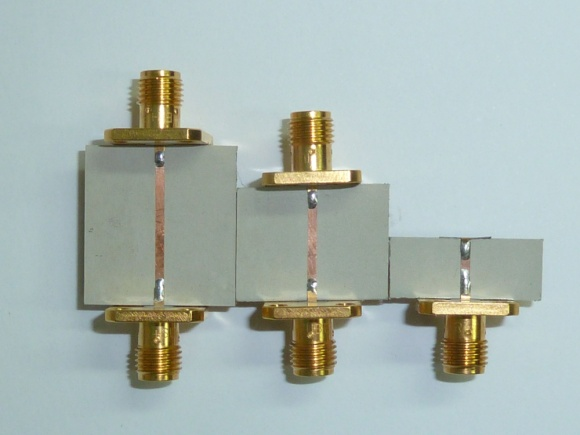
\includegraphics[width=0.4\columnwidth]{fig9a}
\label{f9a}}\hfill
\subfigure[]{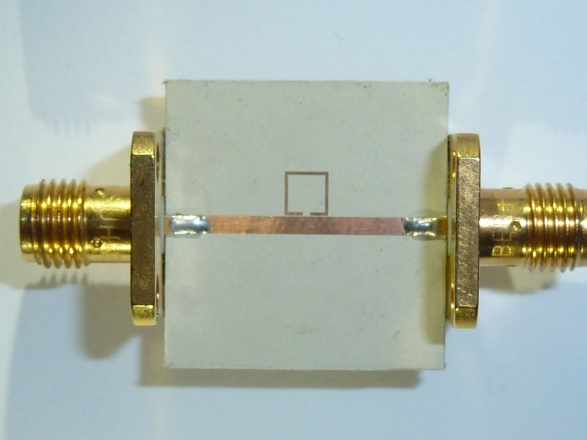
\includegraphics[width=0.4\columnwidth]{fig9b}
\label{f9b}}
\caption{(a) Фабриковани наменски пројектовани LRL калибрациони сет за мерење $S$-параметара на референтним равнима и (б) микрострип вод оптерећен СРР-ом са паралелним процепом ближе воду.} 
\label{f9}
\end{figure}
%%%%%%%%%%%%%%%%%%%%%%%%%%%%%%%%%%%%%%%%%%%%%%%%%%%%%%%%%%%%%%%%%%%%%%%%%%%%%%%%%
Како би се валидирали предложени еквивалентни модели и екстракција њихових параметара, биће упоређене магнитуде и фазе $Ѕ$-параметара добијених мерењем, симулацијама и на основу еквивалентних шема. Симулације су вршене коришћењем идеализованих материјала без губитака, пошто и еквивалентне шеме не укључују губитке. Ипак, одређени губици у симулацијама и мерењима су ипак присутни услед зрачења. Наравно, мерења укључују и губитке у металима и диелектрицима. Све структуре су симулиране у програму WIPL-D~\cite{bib21}, и резултати су деембедовани на референтним равнима, означеним на \Fig{f1}. Измерени $Ѕ$-параметри су такође деембедовани на референтним равнима коришћењем LRL (Line-Reflect-Line) калибрационог сета приказаног на \Fig{f9a}, на анализатору мрежа Anritsu ME7838A. Фабриковани прототип микрострип вода оптерећеног са једним СРР-ом са паралелним процепом ближе воду приказан је на \Fig{f9b}.

%%%%%%%%%%%%%%%%%%%%%%%%%%%%%%%%%%%%%%%%%%%%%%%%%%%%%%%%%%%%%%%%%%%%%%%%%%%%%%%%%
\subsection{СРР-ови са паралелним процепом}
%%%%%%%%%%%%%%%%%%%%%%%%%%%%%%%%%%%%%%%%%%%%%%%%%%%%%%%%%%%%%%%%%%%%%%%%%%%%%%%%%

%%%%%%%%%%%%%%%%%%%%%%%%%%%%%%%%%%%%%%%%%%%%%%%%%%%%%%%%%%%%%%%%%%%%%%%%%%%%%%%%%
\begin{figure}[!t]
\centering
\subfigure[]{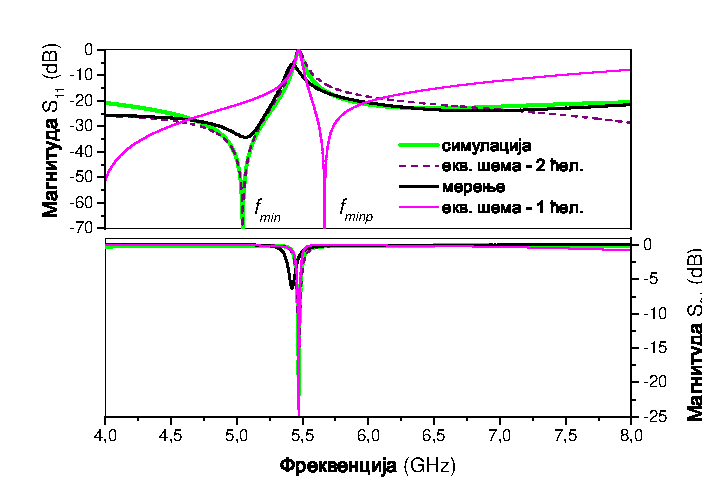
\includegraphics[width=\SirB]{enhmod_slike/fig10a}
\label{f10a}}
\subfigure[]{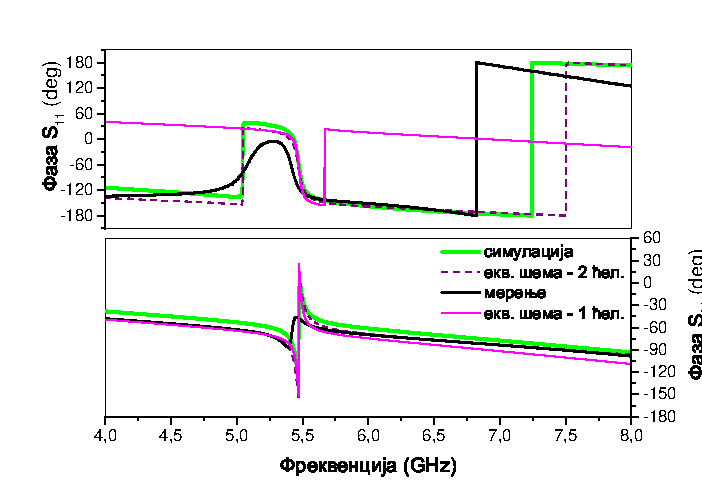
\includegraphics[width=\SirB]{enhmod_slike/fig10b}
\label{f10b}}
\caption{Поређење магнитуда (а) и фаза (б) за $Ѕ$-параметре добијене мерењем, симулацијом и на основу еквивалентне шеме са једном и две П-ћелије за конфигурацију са \Fig{f3a}.}\label{f10}
\end{figure}
%%%%%%%%%%%%%%%%%%%%%%%%%%%%%%%%%%%%%%%%%%%%%%%%%%%%%%%%%%%%%%%%%%%%%%%%%%%%%%%%%
%%%%%%%%%%%%%%%%%%%%%%%%%%%%%%%%%%%%%%%%%%%%%%%%%%%%%%%%%%%%%%%%%%%%%%%%%%%%%%%%%
\begin{figure}[!t]
\centering
\subfigure[]{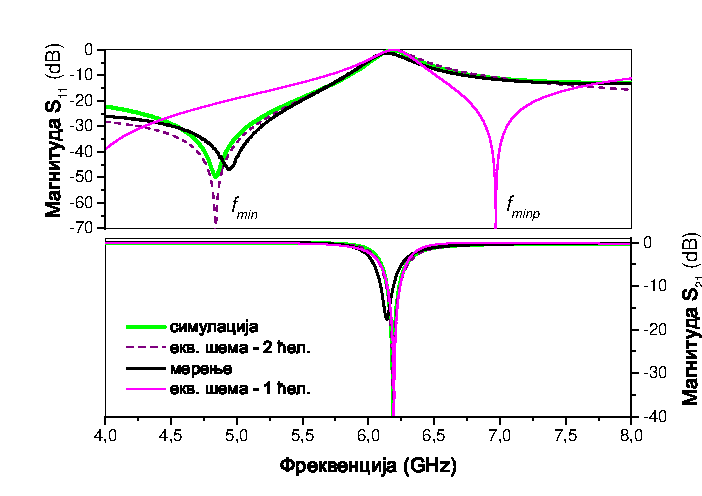
\includegraphics[width=\SirB]{enhmod_slike/fig11a}
\label{f11a}}
\subfigure[]{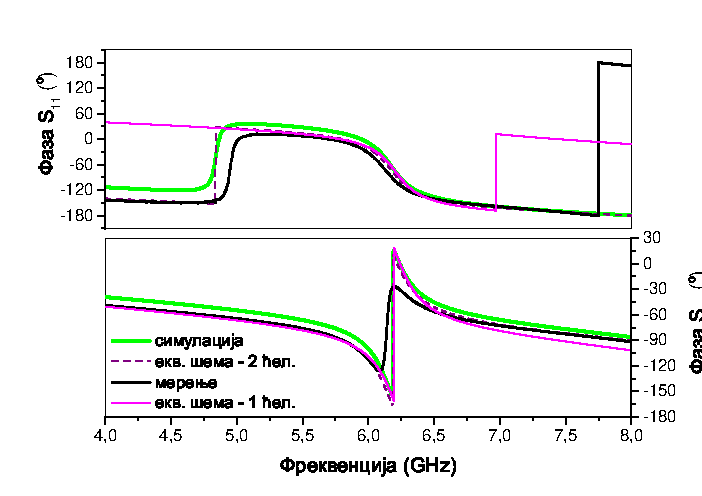
\includegraphics[width=\SirB]{enhmod_slike/fig11b}
\label{f11b}}
\caption{Поређење магнитуда (а) и фаза (б) за $Ѕ$-параметре добијене мерењем, симулацијом и на основу еквивалентне шеме са једном и две П-ћелије за конфигурацију са \Fig{f3c}.} 
\label{f11}
\end{figure}
%%%%%%%%%%%%%%%%%%%%%%%%%%%%%%%%%%%%%%%%%%%%%%%%%%%%%%%%%%%%%%%%%%%%%%%%%%%%%%%%%

Резултати добијени мерењем, симулацијом и анализом помоћу еквивалентне шеме коришћењем две П-ћелије [\Fig{f3f}] за структуре са сл.~\ref{f3a} и \ref{f3c} приказане су на сл.~\ref{f10} и~\ref{f11}, респективно. Резултати се међусобно добро слажу у целом опсегу од 4 до 8 GHz. Мања одступања у магнитуди између еквивалентне шеме и мерења на \Fig{f10} налазе се на крају опсега, и могу се приписати присуству паразитног минимума $S_{11}$. Фреквенција овог минимума је око $8.8\,$GHz услед релативно слабе спреге (упоредити са \Fig{f5}). Насупрот томе, резултати добијени са еквивалентном шемом која користи једну ћелију [\Fig{f3e}] показују велико неслагање са симулацијама и мерењима, без обзира на вредност $k_m$. Заправо, овај поједностављени модел је тачан само на резонантној учестаности и у непосредној околини. Први минимум $S_{11}$ јавља се на далеко нижој учестаности од измерене, и није могуће преклопити их за било коју реалну вредност $k_m$, у складу са~(3). Коефицијенти спреге за еквивалентну шему са једном ћелијом добијени су поступком фитовања и њихове вредности су $k_m=0.1$ за \Fig{f10} и $k_m=0.23$ за \Fig{f11}, за СРР са процепом даље од вода.

%\begin{figure}[!t]
%\centering
%\subfigure[]{\includegraphics[width=0.48\columnwidth]{fig12a}
%\label{f12a}}\hfill
%\subfigure[]{\includegraphics[width=0.48\columnwidth]{fig12b}
%\label{f12b}}
%\caption{Comparison of magnitudes (a) and phases (b) of $S$-parameters obtained by full-wave
%simulations and equivalent circuit analysis with one and two $\Pi$-cells for the configuration
%in \Fig{f3b}.}
%\label{f12}
%\end{figure}
%\sout{To demonstrate that the same two-cells equivalent circuit [\Fig{f3f}] can be used to
%model the microstrip line loaded with two SRRs [\Fig{f3b}] we compare the results given by a
%full-wave simulation and equivalent circuit model in \Fig{f12}. The discrepancy at the end of
%the band is caused again by the presence of the second SRR resonance. Once more, the circuit
%with one cell is unable to achieve good matching over a wide frequency band, being accurate
%only around the resonance. In this last model, the value of magnetic coupling obtained by
%fitting is $k_m=0.135$.}

%%%%%%%%%%%%%%%%%%%%%%%%%%%%%%%%%%%%%%%%%%%%%%%%%%%%%%%%%%%%%%%%%%%%%%%%%%
\subsection{Микрострип вод са два СРР-а са асиметричним процепима}
%%%%%%%%%%%%%%%%%%%%%%%%%%%%%%%%%%%%%%%%%%%%%%%%%%%%%%%%%%%%%%%%%%%%%%%%%%

%%%%%%%%%%%%%%%%%%%%%%%%%%%%%%%%%%%%%%%%%%%%%%%%%%%%%%%%%%%%%%%%%%%%%%%%%%
\begin{figure}[!t]
\centering
\subfigure[]{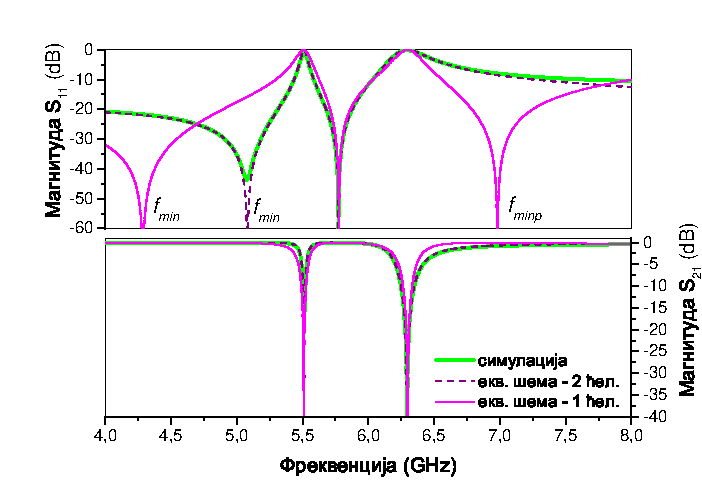
\includegraphics[width=\SirB]{enhmod_slike/fig13a}
\label{f13a}}
\subfigure[]{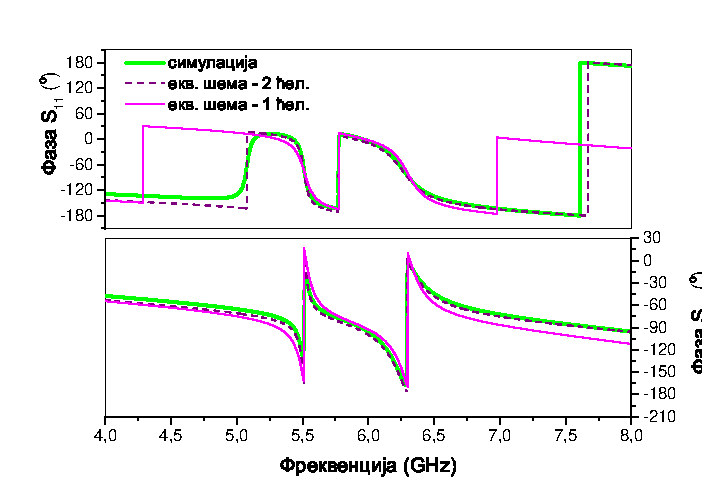
\includegraphics[width=\SirB]{enhmod_slike/fig13b}
\label{f13b}}
\caption{Поређење магнитуда (а) и фаза (б) за $Ѕ$-параметре добијене мерењем, симулацијом и на основу еквивалентне шеме са једном и две П-ћелије за конфигурацију са \Fig{f6a}.} 
\label{f13}
\end{figure}
%%%%%%%%%%%%%%%%%%%%%%%%%%%%%%%%%%%%%%%%%%%%%%%%%%%%%%%%%%%%%%%%%%%%%%%%%%
Поређење између симулације и еквивалентне шеме са једном и две ћелије, за микрострип вод оптерећен са два СРР-а са асиметричним процепима (један ближе воду, други даље од њега), дато је на \Fig{f13}. За случај са шеме са две ћелије, може се видети скоро савршено слагање, и у магнитуди и у фази, у целом опсегу од 4 до 8 GHz. 

За коло са једном ћелијом, добро поклапање се добија само око другог минимума, за коефицијенте спреге $k_{m1}=0.16$ и $k_{m2}=0.18$, што није очекивано, с обзиром да су спрегнуте гране СРР-ова веома различите (са и без процепа). Може се видети да је око друге резонансе неслагање не само у $Ѕ_{11}$, већ и у $Ѕ_{21}$, пошто није изводљиво померити трећи минимум ка вишој фреквенцији. Такође, први минимум $Ѕ_{11}$ није уопште могуће поклопити са колом са једном ћелијом, као што је предвиђено у секцији~\ref{sec3:2}. 

%%%%%%%%%%%%%%%%%%%%%%%%%%%%%%%%%%%%%%%%%%%%%%%%%%%%%%%%%%%%%%%%%%%%%%%%%%
\subsection{СРР-ови са нормалним процепом у односу на вод}
%%%%%%%%%%%%%%%%%%%%%%%%%%%%%%%%%%%%%%%%%%%%%%%%%%%%%%%%%%%%%%%%%%%%%%%%%%

%%%%%%%%%%%%%%%%%%%%%%%%%%%%%%%%%%%%%%%%%%%%%%%%%%%%%%%%%%%%%%%%%%%%%%%%%%
\begin{figure}[!t]
\centering
\subfigure[]{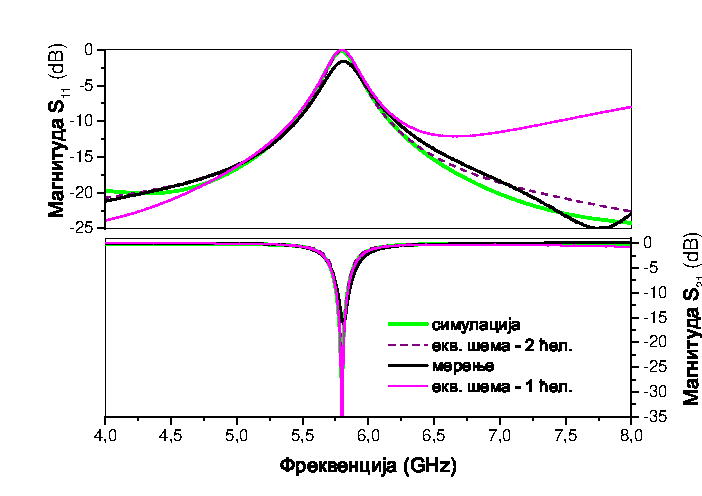
\includegraphics[width=\SirB]{enhmod_slike/fig14a}
\label{f14a}}
\subfigure[]{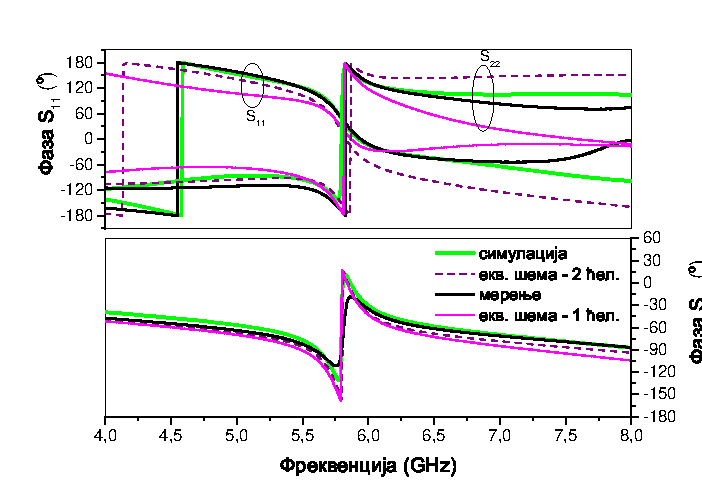
\includegraphics[width=\SirB]{enhmod_slike/fig14b}
\label{f14b}}
\caption{Поређење магнитуда (а) и фаза (б) за $Ѕ$-параметре добијене мерењем, симулацијом и на основу еквивалентне шеме са једном и две П-ћелије за конфигурацију са \Fig{f7a}.}
\label{f14}
\end{figure}
%%%%%%%%%%%%%%%%%%%%%%%%%%%%%%%%%%%%%%%%%%%%%%%%%%%%%%%%%%%%%%%%%%%%%%%%%%
Како би се показале предности унапређене шеме [\Fig{f7c}] у односу на модел са једном ћелијом за СРР са нормалним процепом [\Fig{f7a}], на \Fig{f14} упоређене су магнитуде и фазе $Ѕ$-параметара добијених мерењем, симулацијом и еквивалентном шемом са једном и две П-ћелије. Још једном, резултати за две ћелије су у веома добром слагању са симулацијама и мерењима у целом опсегу од 4 до 8 GHz. Треба приметити да у овом случају не постоји минимум рефлексије испод резонансе СРР-а, као у случајевима са паралелним процепом. Иако је структура асиметрична, само магнитуда $Ѕ_{11}$ је приказана (разлика са $Ѕ_{22}$ је изражена само у фази). Еквивалентна шема са једном ћелијом се сада понаша много боље него у случајевима са паралелним процепом, али предложена шема са две ћелије је ипак боља у ширем опсегу. Екстраховани параметри за модел са једном ћелијом су $k_m=0.28$, $C_m=0.062\,\mathrm{pF}$.

%%%%%%%%%%%%%%%%%%%%%%%%%%%%%%%%%%%%%%%%%%%%%%%%%%%%%%%%%%%%%%%%%%%%%%%%%%
\begin{figure}[!t]
\centering
\subfigure[]{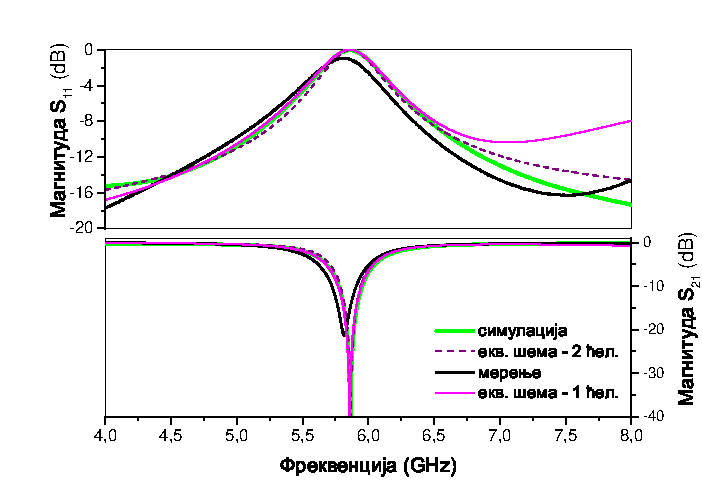
\includegraphics[width=\SirB]{enhmod_slike/fig15a}
\label{f15a}}
\subfigure[]{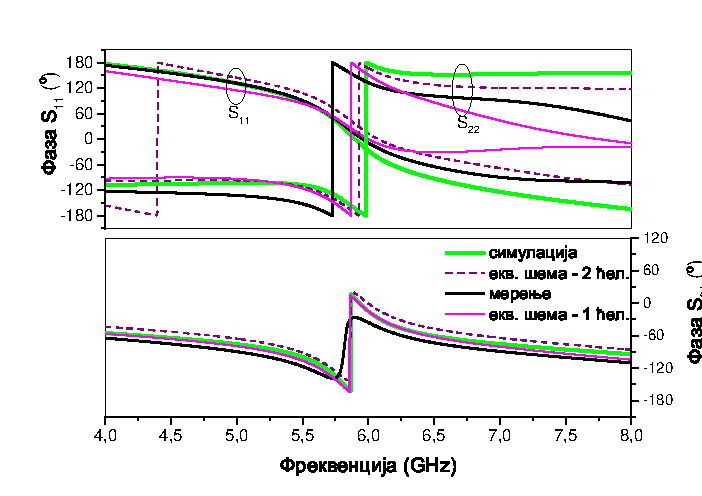
\includegraphics[width=\SirB]{enhmod_slike/fig15b}
\label{f15b}}
\caption{Поређење магнитуда (а) и фаза (б) за $Ѕ$-параметре добијене мерењем, симулацијом и на основу еквивалентне шеме са једном и две П-ћелије за конфигурацију са \Fig{f7b}.}
\label{f15}
\end{figure}
%%%%%%%%%%%%%%%%%%%%%%%%%%%%%%%%%%%%%%%%%%%%%%%%%%%%%%%%%%%%%%%%%%%%%%%%%%
Резултати симулације и анализе помоћу еквивалентне шеме са једном и две П-ћелије за конфигурацију са \Fig{f7b} приказани су на \Fig{f15}. Резултати за две ћелије су у веома добром слагању са симулацијом. Модел са једном ћелијом одговара симулацији у ширем опсегу него у случају само једног СРР-а, и слагање је добро до \SI{7.5}{\giga\hertz}. Екстраховани параметри кола за шему са једном ћелијом су $k_m=0.39$ и $C_m=0.095\, \mathrm{pF}$.

%%%%%%%%%%%%%%%%%%%%%%%%%%%%%%%%%%%%%%%%%%%%%%%%%%%%%%%%%%%%%%%%%%%%%%%%%%
\subsection{Каскадирани СРР-ови са процепом паралелним воду}
%%%%%%%%%%%%%%%%%%%%%%%%%%%%%%%%%%%%%%%%%%%%%%%%%%%%%%%%%%%%%%%%%%%%%%%%%%

%%%%%%%%%%%%%%%%%%%%%%%%%%%%%%%%%%%%%%%%%%%%%%%%%%%%%%%%%%%%%%%%%%%%%%%%%%
\begin{figure}[!t]
\centering
\subfigure[]{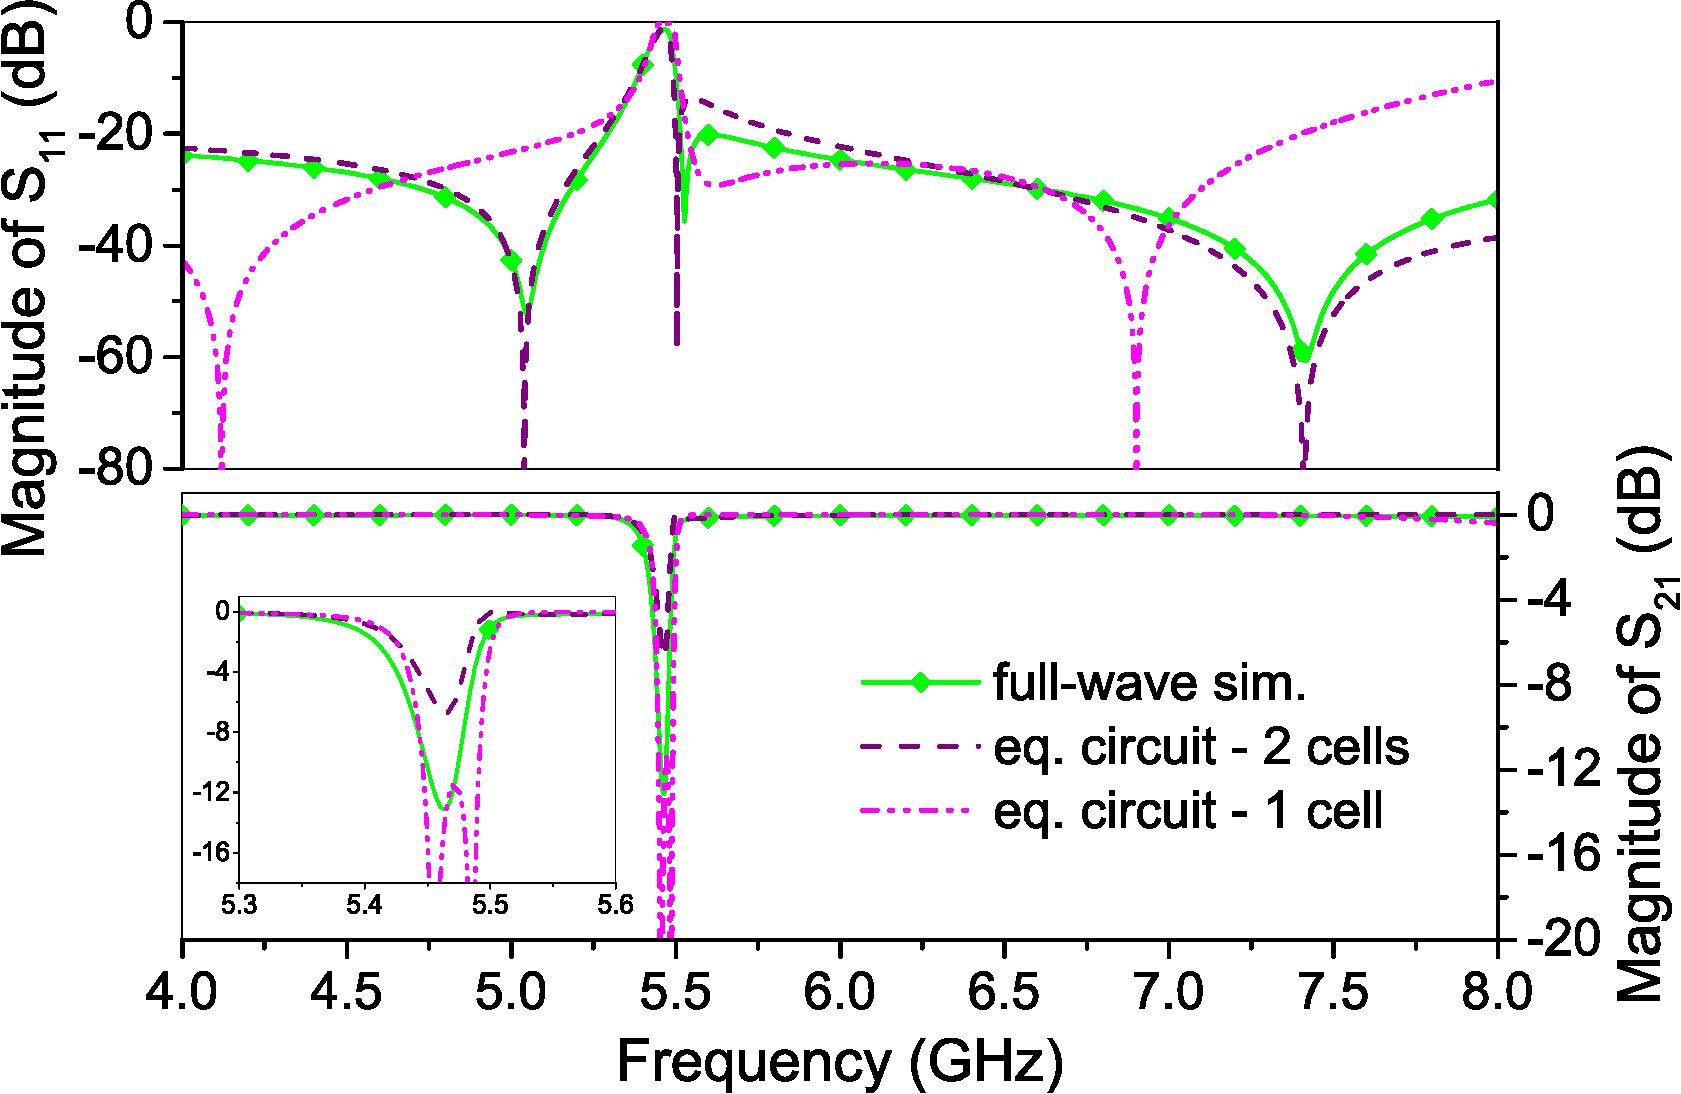
\includegraphics[width=\SirB]{fig16a}
\label{f16a}}
\subfigure[]{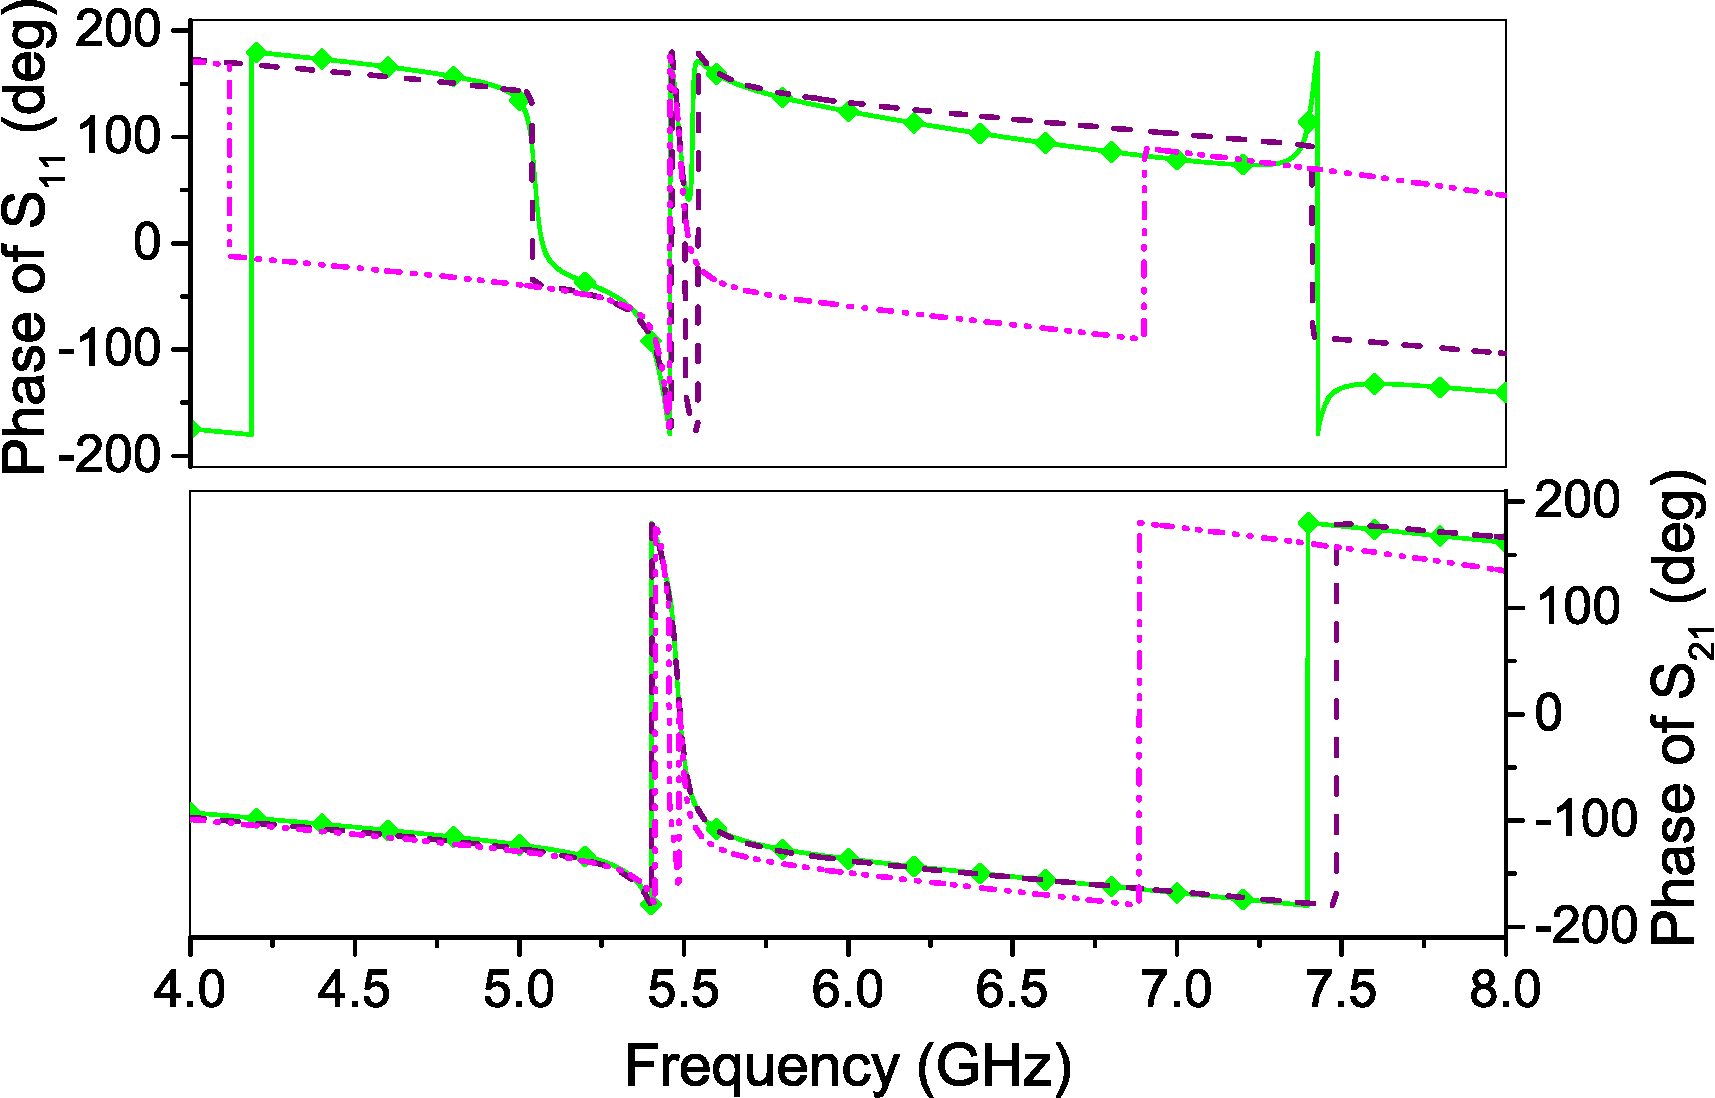
\includegraphics[width=\SirB]{fig16b}
\label{f16b}}
\caption{Поређење магнитуда (а) и фаза (б) за $Ѕ$-параметре добијене мерењем, симулацијом и на основу еквивалентне шеме са једном и две П-ћелије за конфигурацију са \Fig{fk}, за растојање $D=0.5\,\mathrm{mm}$.}
\label{f16}
\end{figure}
%%%%%%%%%%%%%%%%%%%%%%%%%%%%%%%%%%%%%%%%%%%%%%%%%%%%%%%%%%%%%%%%%%%%%%%%%%
Резултати симулације и еквивалентне шеме са једном и две П-ћелије за конфигурацију са \Fig{fk}, за растојање између резонатора $D=0.5\,\mathrm{mm}$, приказани су на \Fig{f16}. Веома добро слагање добијено је у целом опсегу од интереса, и у магнитуди и у фази $Ѕ$-параметара, за модел са две П-ћелије. Насупрот томе, модел са једном П-ћелијом није у стању да поклопи рефлексију, осим у уском опсегу око резонансе. Вредности коефицијената спреге добијене су фитовањем, и износе $k_m=0.1$ и $k_{mc}=0.015$.

%%%%%%%%%%%%%%%%%%%%%%%%%%%%%%%%%%%%%%%%%%%%%%%%%%%%%%%%%%%%%%%%%%%%%%%%%%
\section{Закључак}
%%%%%%%%%%%%%%%%%%%%%%%%%%%%%%%%%%%%%%%%%%%%%%%%%%%%%%%%%%%%%%%%%%%%%%%%%%
Предложена је унапређена еквивалентна шема за микрострип вод оптерећен сплит-ринг резонаторима. Различите оријентације СРР-а у односу на вод су анализиране: са паралелним процепом ближе и даље воду, као и са нормалним процепом. Штампани вод може бити спрегнут са једним СРР-ом са једне стране, или са два СРР-а постављена симетрично/асиметрично са обе стране вода. Овакве структуре испољавају одзив филтра непропусника опсега, али се предложене еквивалентне шеме лако могу модификовати у пропуснике опсега додавањем паралелне индуктивности.

Без обзира да ли је у питању структура са једним или два симетрична СРР-а, користи се иста еквивалентна шема, само са различитим параметрима. Неки од њих се одређују на основу модела вишепроводничког вода ($L$, $C$, $L_s$) док се преостали ($C_s$ и $k_m$) добијају на основу аналитичких израза који их повезују са карактеристичним фреквенцијама -- резонансом и минимумом коефицијента рефлексије, добијеним из симулације. Једини параметар који је неопходно оптимизовати јесте електрична спрега присутна у случају СРР-а са нормалним процепом.

Најважнија предност предложеног модела са две ћелије јесте приближно двоструко већи опсег у коме је могуће преклопити минимум рефлексије добијен из симулације. Ово је постигнуто без повећања параметара кола у односу на модел са једном ћелијом. Такође, унапређена еквивалентна шема боље апроксимира дистрибуирану природу вода, и помера паразитни минимум рефлексије изнад резонансе СРР-а на значајно више фреквенције, у поређењу са моделом са једном ћелијом. Због свега тога, фреквенцијски опсег са добрим поклапањем је значајно увећан.

Више узорака је фабриковано и измерено како би се валидирала процедура екстракције параметара. Врло добро слагање између измерених и симулираних $Ѕ$-параметара и предложене унапређене шеме добијено је у широком фреквенцијском опсегу, и у магнитуди и у фази. Насупрот томе, показано је да конвенционални модел са једном ћелијом ради добро само у уском опсегу. Предложени модел се лако примењује на каскадиране структуре, као што је демонстрирано са две јединичне ћелије са различитим међусобним растојањима. Каскадирани модел је валидиран помоћу симулације, и веома добро слагање је добијено.
\begin{thebibliography}{21}

\bibitem{bib1}
A. Lay, T. Itoh, and C. Caloz, ``Composite right/left-handed transmission line metamaterials,''
\emph{IEEE Microw. Mag.}, vol. 5, no. 3, pp. 34-50, 2004. 
\bibitem{bib2} A. K. Iyer and G. V. Eleftheriades, ``Negative refractive index metamaterials supporting 2-D waves,'' in \emph{Proc. IEEE MTT Int. Symp.}, 2002, vol. 2, pp. 412-415.
\bibitem{bib3} C. Caloz and T. Itoh, ``Application of the transmission line theory of left-handed (LH) materials to the realization of a microstrip LH transmission line,'' in \emph{Proc. IEEE-AP-S USNC/URSI National Radio Science Meeting}, 2002, vol. 2, pp. 412-415. 
\bibitem{bib4} A. A. Oliner, ``A periodic-structure negative-refractive-index medium without resonant elements,'' in \emph{URSI Dig., IEEE-AP-S USNC/URSI National Radio Science Meeting}, 2002, vol. 2, pp.41.
\bibitem{bib5} C. Caloz and T. Itoh, \emph{Electromagnetic Metamaterials: Transmission Line Theory and Microwave Applications}, Wiley-IEEE Press, 2006.
\bibitem{bib6} J. Garc\'{i}a-Garc\'{i}a, J. Bonache, I. Gil, F. Mart\'{i}n, M.C. Velazquez-Ahumada, and J. Martel, ``Miniaturized microstrip and CPW filters using coupled metamaterial resonators,'' \emph{IEEE Trans. Microw. Theory Techn.}, vol. 54, no. 6, pp. 2628-2635, June 2006.
\bibitem{bib7} J. Naqui, M. Dur\'{a}n-Sindreu, and F. Mart\'{i}n, ``Alignment and Position Sensors Based on Split Ring Resonators,'' \emph{Sensors}, vol. 12, no. 9, pp. 11790-11797, September 2012
\bibitem{bib8} F. J. Herraiz-Mart\'{i}nez, F. Paredes, G. Zamora, F. Mart\'{i}n, and J. Bonache, ``Printed Magnetoinductive-Wave (MIW) Delay Lines for Chipless RFID Applications," \emph{IEEE Trans. Antennas Propag.}, vol. 60, no. 11, pp. 5075-5082, November 2012.
\bibitem{bib9} V. Milosevic, B. Jokanovic, and B. Kolundzija, ``Microwave stereometamaterials and parameter extraction,'' \emph{Metamaterials’2010: The Fourth International Congress on Advanced Electromagnetic Materials in Microwaves and Optics}, pp. 474-477, Karlsruhe, Germany, 13-16 September 2010.
\bibitem{bib10} R. Bojanic, B. Jokanovic, and V. Milosevic, ``Multiband Delay Lines with Reconfigurable Split-Ring Resonators,'' \emph{10th International Conference on Telecommunications in Modern Satellite, Cable and Broadcasting Services, TELSIKS2011}, pp. 31-34, Nis, Serbia, October 5-8, 2011.
\bibitem{bib11} N. Boskovic, B. Jokanovic, and A. Nesic, ``Compact frequency scanning antenna array with SRR phase shifters,'' \emph{11th International Conference on Telecommunications in Modern Satellite, Cable and Broadcasting Services, TELSIKS2013}, pp.437-439, Nis, Serbia, October 16-19, 2013.
\bibitem{bib12} J. D. Baena, J. Bonache, F. Martin, R. Marques, F. Falcone, T. Lepetegi, M. Laso, J. Garcia-Garcia, I. Gil, M. F. Portillo, and M. Sorolla, ``Equivalent-Circuit Models for Split-Ring Resonators and Complementary Split-Ring Resonators Coupled to Planar Transmission Lines,'' \emph{IEEE Trans. Microw. Theory Techn.}, vol. 53, no. 4, pp. 1451-1461, Apr 2005.
\bibitem{bib13} F. Aznar, M. Gil, J. Bonache, L. Jelinek,  J. D. Baena,  R. Marqu\'{e}s, and F. Mart\'{i}n, ``Characterization of miniaturized metamaterial resonators coupled to planar transmission lines through parameter extraction,`` \emph{Journal of Applied Physics}, vol. 104, 114501, December 2008.
\bibitem{bib14} F. Falcone, T. Lepetegi, J.D. Baena, R. Marqu\'{e}s, F. Mart\'{i}n, and M. Sorolla, 
``Effective negative-epsilon stopband microstrip lines based on complementary split ring resonators,`` \emph{IEEE Microw. Wireless Compon. Lett.}, vol. 14, pp. 280-282, June 2004.
\bibitem{bib15} V. Crnojevic-Bengin, V. Radonic, and B. Jokanovic, ''Fractal Geometries of Complementary Split-Ring Resonators,'' \emph{IEEE Trans. Microwave Theory Techn.}, vol. 56, no. 10, pp. 2312-2321, Oct 2008.
\bibitem{bib16} I. Gil, J. Bonache, J. Garc\'{i}a-Garc\'{i}a F. Falcone, and F. Mart\'{i}n, ``Metamaterials in Microstrip Technology for Filter Applications,'' \emph{Proc. of the APS-URSI}, Washington (USA), July 2005.
\bibitem{bib17} J. Naqui, M. Dur\'{a}n-Sindreu, and F. Mart\'{i}n, ``Modeling Split-Ring Resonator (SRR) and Complementary Split-Ring Resonator (CSRR) Loaded Transmission Lines Exhibiting Cross-Polarization Effects,'' \emph{IEEE Antennas Wireless Propag. Lett.}, vol. 12, pp. 178-181, March 2013.
\bibitem{bib18} J.S. Hong and M.J. Lancaster, ``Couplings of Microstrip Square Open-Loop Resonators for Cross-Coupled Planar Microwave Filters,'' \emph{IEEE Trans. Microw. Theory Techn.}, vol. 44, no. 12, pp. 2099-2109, Dec 1996.
\bibitem{bib19} A.R. Djordjevic, M.B. Bazdar, T.K. Sarkar, and R.F. Harrington, \emph{LINPAR for Windows: Matrix Parameters for Multiconductor Transmission Lines, Software and User’s Manual}, Norwood, USA: Artech House, 1995.
\bibitem{bib20} E. A. Guillemin, \emph{Synthesis of Passive Networks: Theory and Methods Appropriate to the Realization and Approximation Problems}, p207, Krieger Publishing, 1977, ISBN 0-88275-481-5.
\bibitem{bib21} WIPL-D Pro v8.0, \emph{Software and User’s Manual}, WIPL-D d.o.o., Belgrade, 2010.
\end{thebibliography}

\end{document}


